\documentclass{article}
\usepackage{amsmath}
\usepackage{fullpage}
%\usepackage{graphicx}
\usepackage{tikz}
% \allowdisplaybreaks
\usepackage[aux]{rerunfilecheck}

\newcommand{\ds}{\displaystyle}

% Macros for MATH 110 course dates

\newcommand{\commonTheme}{metropolis}
\newcommand{\commonColorTheme}{metropolis}

\newcommand{\commonAuthor}{Edward Doolittle}
\newcommand{\commonInstitute}{Department of Indigenous Knowledge and
  Science \\ First Nations University of Canada}
\newcommand{\commonCourse}{MATH 110 Calculus I}
\newcommand{\commonTerm}{202510}
\newcommand{\commonDate}{January 6, 2025}

% Review Material

% Lab 0
\newcommand{\commonEventNegativeOne}{LabNegativeOne}
\newcommand{\commonDateLabNegativeOne}{Monday, January 6, 2025}
\newcommand{\commonTitleLabNegativeOne}{MATH 110 Lab 0}
\newcommand{\commonSubtitleLabNegativeOne}{No Lab; Course Opens}

% Section 001
\newcommand{\commonEventZeroZeroOne}{ZeroZeroOne}
\newcommand{\commonDateZeroZeroOne}{Tuesday, January 7, 2025}
\newcommand{\commonTitleZeroZeroOne}{MATH 110 Review 0.1}
\newcommand{\commonSubtitleZeroZeroOne}{Review of Algebra}
\newcommand{\commonPSTitleZeroZeroOne}{MATH 110 Review Problem Set 0.1}

% Section 00A
\newcommand{\commonEventZeroZeroA}{ZeroZeroA}
\newcommand{\commonDateZeroZeroA}{Tuesday, January 7, 2025}
\newcommand{\commonTitleZeroZeroA}{MATH 110 Review 0.A}
\newcommand{\commonSubtitleZeroZeroA}{Review of Inequalities and
  Absolute Values}
\newcommand{\commonPSTitleZeroZeroA}{MATH 110 Review Problem Set 0.A}

% Section 00B
\newcommand{\commonEventZeroZeroB}{ZeroZeroB}
\newcommand{\commonDateZeroZeroB}{Tuesday, January 7, 2025}
\newcommand{\commonTitleZeroZeroB}{MATH 110 Review 0.B}
\newcommand{\commonSubtitleZeroZeroB}{Review of Coordinate Geometry
  and Lines}
\newcommand{\commonPSTitleZeroZeroB}{MATH 110 Review Problem Set 0.B}

% Section 00C
\newcommand{\commonEventZeroZeroC}{ZeroZeroC}
\newcommand{\commonDateZeroZeroC}{Thursday, January 9, 2025}
\newcommand{\commonTitleZeroZeroC}{MATH 110 Review 0.C}
\newcommand{\commonSubtitleZeroZeroC}{Review of Graphs of Second
  Degree Equations}
\newcommand{\commonPSTitleZeroZeroC}{MATH 110 Review Problem Set 0.C}

% Section 00D
\newcommand{\commonEventZeroZeroD}{ZeroZeroD}
\newcommand{\commonDateZeroZeroD}{Thursday, January 9, 2025}
\newcommand{\commonTitleZeroZeroD}{MATH 110 Review 0.D}
\newcommand{\commonSubtitleZeroZeroD}{Review of Trigonometry}
\newcommand{\commonPSTitleZeroZeroD}{MATH 110 Review Problem Set 0.D}

% Section 011
\newcommand{\commonEventZeroOneOne}{ZeroOneOne}
\newcommand{\commonDateZeroOneOne}{Thursday, January 9, 2025}
\newcommand{\commonTitleZeroOneOne}{MATH 110 Review 1.1}
\newcommand{\commonSubtitleZeroOneOne}{Review of Functions}
\newcommand{\commonPSTitleZeroOneOne}{MATH 110 Review Problem Set 1.1}


% Main Course

% Lab 1
\newcommand{\commonEventZero}{LabZero}
\newcommand{\commonDateLabZero}{Monday, January 13, 2025}
\newcommand{\commonTitleLabZero}{MATH 110 Lab 1}
\newcommand{\commonSubtitleLabZero}{Quiz 0: STACK, Onboarding}

% Section 1.4
\newcommand{\commonEventOne}{ZeroOneFour}
\newcommand{\commonDateZeroOneFour}{Tuesday, January 14, 2025}
\newcommand{\commonTitleZeroOneFour}{MATH 110 Lecture 1.4}
\newcommand{\commonSubtitleZeroOneFour}{The Tangent and Velocity Problems}
\newcommand{\commonPSTitleZeroOneFour}{MATH 110 Problem Set 1.4}

% Section 1.5
\newcommand{\commonEventTwo}{ZeroOneFive}
\newcommand{\commonDateZeroOneFive}{Thursday, January 16, 2025}
\newcommand{\commonTitleZeroOneFive}{MATH 110 Lecture 1.5}
\newcommand{\commonSubtitleZeroOneFive}{The Limit of a Function}
\newcommand{\commonPSTitleZeroOneFive}{MATH 110 Problem Set 1.5}

% Lab 2
\newcommand{\commonEventThree}{LabOne}
\newcommand{\commonDateLabOne}{Monday, January 20, 2025}
\newcommand{\commonTitleLabOne}{MATH 110 Lab 2}
\newcommand{\commonSubtitleLabOne}{Quiz 1: Review}

% Section 1.6
\newcommand{\commonEventFour}{ZeroOneSix}
\newcommand{\commonDateZeroOneSix}{Tuesday, January 21, 2025}
\newcommand{\commonTitleZeroOneSix}{MATH 110 Lecture 1.6}
\newcommand{\commonSubtitleZeroOneSix}{Calculating Limits Using the Limit Laws}
\newcommand{\commonPSTitleZeroOneSix}{MATH 110 Problem Set 1.6}

% Section 1.7
\newcommand{\commonEventFive}{ZeroOneSeven}
\newcommand{\commonDateZeroOneSeven}{(Not covered)}
\newcommand{\commonTitleZeroOneSeven}{MATH 110 Lecture 1.7}
\newcommand{\commonSubtitleZeroOneSeven}{The Precise Definition of a Limit}
\newcommand{\commonPSTitleZeroOneSeven}{MATH 110 Problem Set 1.7}

% Section 1.8
\newcommand{\commonEventSix}{ZeroOneEight}
\newcommand{\commonDateZeroOneEight}{Thursday, January 23, 2025}
\newcommand{\commonTitleZeroOneEight}{MATH 110 Lecture 1.8}
\newcommand{\commonSubtitleZeroOneEight}{Continuity}
\newcommand{\commonPSTitleZeroOneEight}{MATH 110 Problem Set 1.8}

% Lab 3
\newcommand{\commonEventSeven}{LabTwo}
\newcommand{\commonDateLabTwo}{Monday, January 27, 2025}
\newcommand{\commonTitleLabTwo}{MATH 110 Lab 3}
\newcommand{\commonSubtitleLabTwo}{Quiz 2: Sections 1.4, 1.5}

% Section 2.1
\newcommand{\commonEventEight}{ZeroTwoOne}
\newcommand{\commonDateZeroTwoOne}{Tuesday, January 28, 2025}
\newcommand{\commonTitleZeroTwoOne}{MATH 110 Lecture 2.1}
\newcommand{\commonSubtitleZeroTwoOne}{Derivatives and Rates of Change}
\newcommand{\commonPSTitleZeroTwoOne}{MATH 110 Problem Set 2.1}

% Section 2.2
\newcommand{\commonEventNine}{ZeroTwoTwo}
\newcommand{\commonDateZeroTwoTwo}{Thursday, January 30, 2025}
\newcommand{\commonTitleZeroTwoTwo}{MATH 110 Lecture 2.2}
\newcommand{\commonSubtitleZeroTwoTwo}{The Derivative as a Function}
\newcommand{\commonPSTitleZeroTwoTwo}{MATH 110 Problem Set 2.2}

% Lab 4
\newcommand{\commonEventTen}{LabThree}
\newcommand{\commonDateMTOne}{Monday, February 3, 2025} 
\newcommand{\commonDateLabThree}{Monday, February 3, 2025}
\newcommand{\commonTitleLabThree}{MATH 110 Lab 4}
\newcommand{\commonSubtitleLabThree}{Midterm: Review, Chapter 1}

% Section 2.3
\newcommand{\commonEventEleven}{ZeroTwoThree}
\newcommand{\commonDateZeroTwoThree}{Tuesday, February 4, 2025}
\newcommand{\commonTitleZeroTwoThree}{MATH 110 Lecture 2.3}
\newcommand{\commonSubtitleZeroTwoThree}{Differentiation Formulas}
\newcommand{\commonPSTitleZeroTwoThree}{MATH 110 Problem Set 2.3}

% Section 2.4
\newcommand{\commonEventTwelve}{ZeroTwoFour}
\newcommand{\commonDateZeroTwoFour}{Thursday, February 6, 2025}
\newcommand{\commonTitleZeroTwoFour}{MATH 110 Lecture 2.4}
\newcommand{\commonSubtitleZeroTwoFour}{Derivatives of Trigonometric Functions}
\newcommand{\commonPSTitleZeroTwoFour}{MATH 110 Problem Set 2.4}

% Lab 5
\newcommand{\commonEventThirteen}{LabFour}
\newcommand{\commonDateLabFour}{Monday, February 10, 2025}
\newcommand{\commonTitleLabFour}{MATH 110 Lab 5}
\newcommand{\commonSubtitleLabFour}{Quiz 3: Sections 2.1, 2.2}

% Section 2.5
\newcommand{\commonEventFourteen}{ZeroTwoFive}
\newcommand{\commonDateZeroTwoFive}{Tuesday, February 11, 2025}
\newcommand{\commonTitleZeroTwoFive}{MATH 110 Lecture 2.5}
\newcommand{\commonSubtitleZeroTwoFive}{The Chain Rule}
\newcommand{\commonPSTitleZeroTwoFive}{MATH 110 Problem Set 2.5}

% Section 2.6
\newcommand{\commonEventFifteen}{ZeroTwoSix}
\newcommand{\commonDateZeroTwoSix}{Thursday, February 13, 2025}
\newcommand{\commonTitleZeroTwoSix}{MATH 110 Lecture 2.6}
\newcommand{\commonSubtitleZeroTwoSix}{Implicit Differentiation}
\newcommand{\commonPSTitleZeroTwoSix}{MATH 110 Problem Set 2.6}

% Lab 6
\newcommand{\commonEventSixteen}{LabFive}
\newcommand{\commonDateLabFive}{Monday, February 24, 2025}
\newcommand{\commonTitleLabFive}{MATH 110 Lab 6}
\newcommand{\commonSubtitleLabFive}{Quiz 4: Sections 2.3, 2.4}

% Section 2.7
\newcommand{\commonEventSeventeen}{ZeroTwoSeven}
\newcommand{\commonDateZeroTwoSeven}{Tuesday, February 25, 2025}
\newcommand{\commonTitleZeroTwoSeven}{MATH 110 Lecture 2.7}
\newcommand{\commonSubtitleZeroTwoSeven}{Rates of Change in the
  Natural and Social Sciences}
\newcommand{\commonPSTitleZeroTwoSeven}{MATH 110 Problem Set 2.7}

% Section 2.8
\newcommand{\commonEventEighteen}{ZeroTwoEight}
\newcommand{\commonDateZeroTwoEight}{Thursday, February 27, 2025}
\newcommand{\commonTitleZeroTwoEight}{MATH 110 Lecture 2.8}
\newcommand{\commonSubtitleZeroTwoEight}{Related Rates}
\newcommand{\commonPSTitleZeroTwoEight}{MATH 110 Problem Set 2.8}

% Lab 7
\newcommand{\commonEventNineteen}{LabSix}
\newcommand{\commonDateLabSix}{Monday, March 3, 2025}
\newcommand{\commonTitleLabSix}{MATH 110 Lab 7}
\newcommand{\commonSubtitleLabSix}{Quiz 5: Sections 2.5, 2.6}

% Section 3.1
\newcommand{\commonEventTwenty}{ZeroThreeOne}
\newcommand{\commonDateZeroThreeOne}{Tuesday, March 4, 2025}
\newcommand{\commonTitleZeroThreeOne}{MATH 110 Lecture 3.1}
\newcommand{\commonSubtitleZeroThreeOne}{Maximum and Minimum Values}
\newcommand{\commonPSTitleZeroThreeOne}{MATH 11 Problem Set 3.1}

% Section 3.2
\newcommand{\commonEventTwentyOne}{ZeroThreeTwo}
\newcommand{\commonDateZeroThreeTwo}{Thursday, March 6, 2025}
\newcommand{\commonTitleZeroThreeTwo}{MATH 110 Lecture 3.2}
\newcommand{\commonSubtitleZeroThreeTwo}{The Mean Value Theorem}
\newcommand{\commonPSTitleZeroThreeTwo}{MATH 110 Problem Set 3.2}

% Lab 8
\newcommand{\commonEventTwentyTwo}{LabSeven}
\newcommand{\commonDateMTTwo}{Monday, March 10, 2025}
\newcommand{\commonDateLabSeven}{Monday, March 10, 2025}
\newcommand{\commonTitleLabSeven}{MATH 110 Lab 8}
\newcommand{\commonSubtitleLabSeven}{Midterm: Chapter 2}

% Section 3.3
\newcommand{\commonEventTwentyThree}{ZeroThreeThree}
\newcommand{\commonDateZeroThreeThree}{Tuesday, March 11, 2025}
\newcommand{\commonTitleZeroThreeThree}{MATH 110 Lecture 3.3}
\newcommand{\commonSubtitleZeroThreeThree}{How Derivatives Affect the
  Shape of a Graph}
\newcommand{\commonPSTitleZeroThreeThree}{MATH 110 Problem Set 3.3}

% Section 3.4
\newcommand{\commonEventTwentyFour}{ZeroThreeFour}
\newcommand{\commonDateZeroThreeFour}{Thursday, March 13, 2025}
\newcommand{\commonTitleZeroThreeFour}{MATH 110 Lecture 3.4}
\newcommand{\commonSubtitleZeroThreeFour}{Limits at Infinity;
  Horizontal Asymptotes}
\newcommand{\commonPSTitleZeroThreeFour}{MATH 110 Problem Set 3.4}

% Lab 9
\newcommand{\commonEventTwentyFive}{LabEight}
\newcommand{\commonDateLabEight}{Monday, March 17, 2025}
\newcommand{\commonTitleLabEight}{MATH 110 Lab 9}
\newcommand{\commonSubtitleLabEight}{Quiz 6: Sections 3.1, 3.2}

% Section 3.5
\newcommand{\commonEventTwentySix}{ZeroThreeFive}
\newcommand{\commonDateZeroThreeFive}{Tuesday, March 18, 2025}
\newcommand{\commonTitleZeroThreeFive}{MATH 110 Lecture 3.5}
\newcommand{\commonSubtitleZeroThreeFive}{Summary of Curve Sketching}
\newcommand{\commonPSTitleZeroThreeFive}{MATH 110 Problem Set 3.5}

% Section 3.7
\newcommand{\commonEventTwentySeven}{ZeroThreeSeven}
\newcommand{\commonDateZeroThreeSeven}{Thursday, March 20, 2025}
\newcommand{\commonTitleZeroThreeSeven}{MATH 110 Lecture 3.7}
\newcommand{\commonSubtitleZeroThreeSeven}{Optimization Problems}
\newcommand{\commonPSTitleZeroThreeSeven}{MATH 110 Problem Set 3.7}

% Lab 10
\newcommand{\commonEventTwentyEight}{LabNine}
\newcommand{\commonDateLabNine}{Monday, March 24, 2025}
\newcommand{\commonTitleLabNine}{MATH 110 Lab 10}
\newcommand{\commonSubtitleLabNine}{Quiz 7: Sections 3.3, 3.4}

% Section 4.1
\newcommand{\commonEventTwentyNine}{ZeroFourOne}
\newcommand{\commonDateZeroFourOne}{Tuesday, March 25, 2025}
\newcommand{\commonTitleZeroFourOne}{MATH 110 Lecture 4.1}
\newcommand{\commonSubtitleZeroFourOne}{Areas and Distances}
\newcommand{\commonPSTitleZeroFourOne}{MATH 110 Problem Set 4.1}

% Section 4.2
\newcommand{\commonEventThirty}{ZeroFourTwo}
\newcommand{\commonDateZeroFourTwo}{Thursday, March 27, 2025}
\newcommand{\commonTitleZeroFourTwo}{MATH 110 Lecture 4.2}
\newcommand{\commonSubtitleZeroFourTwo}{The Definite Integral}
\newcommand{\commonPSTitleZeroFourTwo}{MATH 110 Problem Set 4.2}

% Lab 11
\newcommand{\commonEventThirtyOne}{LabTen}
\newcommand{\commonDateLabTen}{Monday, March 31, 2025}
\newcommand{\commonTitleLabTen}{MATH 110 Lab 11}
\newcommand{\commonSubtitleLabTen}{Quiz 8: Sections 3.5, 3.7}

% Section 4.3
\newcommand{\commonEventThirtyTwo}{ZeroFourThree}
\newcommand{\commonDateZeroFourThree}{Tuesday, April 1, 2025}
\newcommand{\commonTitleZeroFourThree}{MATH 110 Lecture 4.3}
\newcommand{\commonSubtitleZeroFourThree}{The Fundamental Theorem of Calculus}
\newcommand{\commonPSTitleZeroFourThree}{MATH 110 Problem Set 4.3}

% Section 4.4
\newcommand{\commonEventThirtyThree}{ZeroFourFour}
\newcommand{\commonDateZeroFourFour}{Thursday, April 3, 2025}
\newcommand{\commonTitleZeroFourFour}{MATH 110 Lecture 4.4}
\newcommand{\commonSubtitleZeroFourFour}{Indefinite Integrals and the
  Net Change Theorem}
\newcommand{\commonPSTitleZeroFourFour}{MATH 110 Problem Set 4.4}

% Lab 12
\newcommand{\commonEventThirtyFour}{LabEleven}
\newcommand{\commonDateLabEleven}{Monday, April 7, 2025}
\newcommand{\commonTitleLabEleven}{MATH 110 Lab 12}
\newcommand{\commonSubtitleLabEleven}{Quiz 9: Sections 4.1, 4.2}

% Section 4.5
\newcommand{\commonEventThirtyFive}{ZeroFourFive}
\newcommand{\commonDateZeroFourFive}{Tuesday, April 8, 2025}
\newcommand{\commonTitleZeroFourFive}{MATH 110 Lecture 4.5}
\newcommand{\commonSubtitleZeroFourFive}{The Substitution Rule}
\newcommand{\commonPSTitleZeroFourFive}{MATH 110 Problem Set 4.5}

% Section 5.1
\newcommand{\commonEventThirtySix}{ZeroFiveOne}
\newcommand{\commonDateZeroFiveOne}{Thursday, April 10, 2025}
\newcommand{\commonTitleZeroFiveOne}{MATH 110 Lecture 5.1}
\newcommand{\commonSubtitleZeroFiveOne}{Areas Between Curves}
\newcommand{\commonPSTitleZeroFiveOne}{MATH 110 Problem Set 5.1}

% Lab 13
\newcommand{\commonEventThirtySeven}{LabTwelve}
\newcommand{\commonDateLabTwelve}{Monday, April 14, 2025}
\newcommand{\commonTitleLabTwelve}{MATH 110 Review Lab}
\newcommand{\commonSubtitleLabTwelve}{Bonus Quiz 10: Sections 4.3, 4.4}

% Final Class
\newcommand{\commonEventThirtyEight}{FinalClass}
\newcommand{\commonDateFinalClass}{Tuesday, April 15, 2025}
\newcommand{\commonTitleFinalClass}{MATH 110 Review Class}
\newcommand{\commonSubtitleFinalClass}{Answer Questions, Review for Exam}

% Final Exam
\newcommand{\commonEventThirtyNine}{Final}
\newcommand{\commonDateFinal}{Thursday, April 22, 2025}
\newcommand{\commonTitleFinal}{MATH 110 Final Exam}
\newcommand{\commonSubtitleFinal}{Comprehensive Exam: All Sections}

% Orphaned -- no longer part of the course

% Section 2.9
\newcommand{\commonDateZeroTwoNine}{Not part of the course}
\newcommand{\commonTitleZeroTwoNine}{MATH 110 Lecture 2.9}
\newcommand{\commonSubtitleZeroTwoNine}{Linear Approximations and Differentials}
\newcommand{\commonPSTitleZeroTwoNine}{MATH 110 Problem Set 2.9}


% % Introduction
% \newcommand{\commonEventOneDate}{Wednesday, September 8, 2010}
% \newcommand{\commonEventOneDesc}{Introduction to the Course}
% \newcommand{\commonDateZeroZeroZero}{September 8, 2010}
% \newcommand{\commonTitleZeroZeroZero}{MATH 104 Introduction}
% \newcommand{\commonSubtitleZeroZeroZero}{Outline of the Course}

% % Lecture 1
% \newcommand{\commonEventTwoDate}{Friday, September 10, 2010}
% \newcommand{\commonEventTwoDesc}{Lecture 1: Algebra}
% \newcommand{\commonDateZeroZeroOne}{September 10, 2010}
% \newcommand{\commonTitleZeroZeroOne}{MATH 104 Lecture 1}
% \newcommand{\commonSubtitleZeroZeroOne}{Review of Algebra}
% % associated evaluation ... factor this out?
% \newcommand{\commonPSTitleZeroZeroOne}{MATH 104 Problem Set 1}
% \newcommand{\commonEvalZeroZeroOne}{Quiz 1}
% \newcommand{\commonEvalDateZeroZeroOne}{Wednesday, September 15, 2010}

% % Lecture 2
% \newcommand{\commonEventThreeDate}{Monday, September 13, 2010}
% \newcommand{\commonEventThreeDesc}{Lecture 2: Appendix A}
% \newcommand{\commonDateZeroZeroA}{September 13, 2010}
% \newcommand{\commonTitleZeroZeroA}{MATH 104 Lecture 2}
% \newcommand{\commonSubtitleZeroZeroA}{Appendix A: Numbers, Inequalities, 
%   and Absolute Values}
% % associated evaluation ... factor this out?
% \newcommand{\commonPSTitleZeroZeroA}{MATH 104 Problem Set 2}
% \newcommand{\commonEvalZeroZeroA}{Quiz 2}
% \newcommand{\commonEvalDateZeroZeroA}{Wednesday, September 22, 2010}

% % Review 1
% \newcommand{\commonEventFourDate}{Wednesday, September 15, 2010}
% \newcommand{\commonEventFourDesc}{Review 1: Review Algebra; Quiz 1; Review Appendix A}
% \newcommand{\commonDateRZeroOne}{September 15, 2010}
% \newcommand{\commonTitleRZeroOne}{MATH 104 Review 1}
% \newcommand{\commonSubtitleRZeroOne}{Review of Algebra, Appendix A}

% % Lecture 3
% \newcommand{\commonEventFiveDate}{Friday, September 17, 2010}
% \newcommand{\commonEventFiveDesc}{Lecture 3: Appendix B}
% \newcommand{\commonDateZeroZeroB}{September 17, 2010}
% \newcommand{\commonTitleZeroZeroB}{MATH 104 Lecture 3}
% \newcommand{\commonSubtitleZeroZeroB}{Appendix B: Coordinate Geometry and Lines}
% % associated evaluation ... factor this out?
% \newcommand{\commonPSTitleZeroZeroB}{MATH 104 Problem Set 3}
% \newcommand{\commonEvalZeroZeroB}{Quiz 2}
% \newcommand{\commonEvalDateZeroZeroB}{Wednesday, September 22, 2010}

% % Lecture 4
% \newcommand{\commonEventSixDate}{Monday, Sepbember 20, 2010}
% \newcommand{\commonEventSixDesc}{Lecture 4: Appendix C}
% \newcommand{\commonDateZeroZeroC}{September 20, 2010}
% \newcommand{\commonTitleZeroZeroC}{MATH 104 Lecture 4}
% \newcommand{\commonSubtitleZeroZeroC}{Appendix C: Graphs of Second-Degree Equations}
% % associated evaluation ... factor this out?
% \newcommand{\commonPSTitleZeroZeroC}{MATH 104 Problem Set 4}
% \newcommand{\commonEvalZeroZeroC}{Midterm 0}
% \newcommand{\commonEvalDateZeroZeroC}{Wednesday, September 29, 2010}

% % Review 2
% \newcommand{\commonEventSevenDate}{Wednesday, September 22, 2010}
% \newcommand{\commonEventSevenDesc}{Review 2: Review Appendix B; Quiz 2; Review Appendix C}
% \newcommand{\commonDateRZeroTwo}{September 22, 2010}
% \newcommand{\commonTitleRZeroTwo}{MATH 104 Review 2}
% \newcommand{\commonSubtitleRZeroTwo}{Review of Appendices B and C}

% % Lecture 5
% \newcommand{\commonEventEightDate}{Friday, September 24, 2010}
% \newcommand{\commonEventEightDesc}{Lecture 5: Appendix D}
% \newcommand{\commonDateZeroZeroD}{September 24, 2010}
% \newcommand{\commonTitleZeroZeroD}{MATH 104 Lecture 5}
% \newcommand{\commonSubtitleZeroZeroD}{Appendix D: Trigonometry}
% % associated evaluation ... factor this out?
% \newcommand{\commonPSTitleZeroZeroD}{MATH 104 Problem Set 5}
% \newcommand{\commonEvalZeroZeroD}{Midterm 0}
% \newcommand{\commonEvalDateZeroZeroD}{Wednesday, September 29, 2010}

% % Lecture 6
% \newcommand{\commonEventNineDate}{Monday, September 27, 2010}
% \newcommand{\commonEventNineDesc}{Lecture 6: Section 1.1}
% \newcommand{\commonDateZeroOneOne}{September 27, 2010}
% \newcommand{\commonTitleZeroOneOne}{MATH 104 Lecture 6}
% \newcommand{\commonSubtitleZeroOneOne}{Section 1.1: Four Ways to Represent a Function}
% % associated evaluation ... factor this out?
% \newcommand{\commonPSTitleZeroOneOne}{MATH 104 Problem Set 6}
% \newcommand{\commonEvalZeroOneOne}{Quiz 3}
% \newcommand{\commonEvalDateZeroOneOne}{Wednesday, October 6, 2010}

% % Review 3
% \newcommand{\commonEventTenDate}{Wednesday, September 29, 2010}
% \newcommand{\commonEventTenDesc}{Review 3: Review Appendix D; 
%   Self-Assessment Midterm 0}
% \newcommand{\commonDateRZeroThree}{September 29, 2010}
% \newcommand{\commonTitleRZeroThree}{MATH 104 Review 3}
% \newcommand{\commonSubtitleRZeroThree}{Review of Appendix D}

% % Lecture 7
% \newcommand{\commonEventElevenDate}{Friday, October 1, 2010}
% \newcommand{\commonEventElevenDesc}{Lecture 7: Section 1.2}
% \newcommand{\commonDateZeroOneTwo}{October 1, 2010}
% \newcommand{\commonTitleZeroOneTwo}{MATH 104 Lecture 7}
% \newcommand{\commonSubtitleZeroOneTwo}{Section 1.2: Mathematical Models: A Catalog of Essential Functions}
% % associated evaluation ... factor this out?
% \newcommand{\commonPSTitleZeroOneTwo}{MATH 104 Problem Set 7}
% \newcommand{\commonEvalZeroOneTwo}{Quiz 3}
% \newcommand{\commonEvalDateZeroOneTwo}{Wednesday, October 6, 2010}

% % Lecture 8
% \newcommand{\commonEventTwelveDate}{Monday, October 4, 2010}
% \newcommand{\commonEventTwelveDesc}{Lecture 8: Section 1.3}
% \newcommand{\commonDateZeroOneThree}{October 4, 2010}
% \newcommand{\commonTitleZeroOneThree}{MATH 104 Lecture 8}
% \newcommand{\commonSubtitleZeroOneThree}{Section 1.3: New Functions from Old Functions}
% % associated evaluation ... factor this out?
% \newcommand{\commonPSTitleZeroOneThree}{MATH 104 Problem Set 8}
% \newcommand{\commonEvalZeroOneThree}{Quiz 4}
% \newcommand{\commonEvalDateZeroOneThree}{Wednesday, October 13, 2010}

% % Review 4
% \newcommand{\commonEventThirteenDate}{Wednesday, October 6, 2010}
% \newcommand{\commonEventThirteenDesc}{Review 4: Review 1.1, 1.2; Quiz 3}
% \newcommand{\commonDateROneOne}{October 6, 2010}
% \newcommand{\commonTitleROneOne}{MATH 104 Review 4}
% \newcommand{\commonSubtitleROneOne}{Reveiw of 1.1, 1.2}

% % Lecture 9
% \newcommand{\commonEventFourteenDate}{Friday, October 8, 2010}
% \newcommand{\commonEventFourteenDesc}{Lecture 9: Section 1.4}
% \newcommand{\commonDateZeroOneFour}{October 8, 2010}
% \newcommand{\commonTitleZeroOneFour}{MATH 104 Lecture 9}
% \newcommand{\commonSubtitleZeroOneFour}{Section 1.4: Graphing Calculators and Computers}
% % associated evaluation ... factor this out?
% \newcommand{\commonPSTitleZeroOneFour}{MATH 104 Problem Set 9}
% \newcommand{\commonEvalZeroOneFour}{Quiz 4}
% \newcommand{\commonEvalDateZeroOneFour}{Wednesday, October 13, 2010}

% % Thanksgiving holiday
% \newcommand{\commonEventFifteenDate}{Monday, October 11, 2010}
% \newcommand{\commonEventFifteenDesc}{No class: Thanksgiving holiday}

% % Review 5
% \newcommand{\commonEventSixteenDate}{Wednesday, October 13, 2010}
% \newcommand{\commonEventSixteenDesc}{Review 5: Review 1.3, 1.4; Quiz 4}
% \newcommand{\commonDateROneTwo}{October 13, 2010}
% \newcommand{\commonTitleROneTwo}{MATH 104 Review 5}
% \newcommand{\commonSubtitleOneRTwo}{Review of 1.3, 1.4}

% % Lecture 10
% \newcommand{\commonEventSeventeenDate}{Friday, October 15, 2010}
% \newcommand{\commonEventSeventeenDesc}{Lecture 10: Section 1.5}
% \newcommand{\commonDateZeroOneFive}{October 15, 2010}
% \newcommand{\commonTitleZeroOneFive}{MATH 104 Lecture 10}
% \newcommand{\commonSubtitleZeroOneFive}{Section 1.5: Exponential Functions}
% % associated evaluation ... factor this out?
% \newcommand{\commonPSTitleZeroOneFive}{MATH 104 Problem Set 10}
% \newcommand{\commonEvalZeroOneFive}{Quiz 5}
% \newcommand{\commonEvalDateZeroOneFive}{Wednesday, October 20, 2010}

% % Lecture 11
% \newcommand{\commonEventEighteenDate}{Monday, October 18, 2010}
% \newcommand{\commonEventEighteenDesc}{Lecture 11: Section 1.6}
% \newcommand{\commonDateZeroOneSix}{October 18, 2010}
% \newcommand{\commonTitleZeroOneSix}{MATH 104 Lecture 11}
% \newcommand{\commonSubtitleZeroOneSix}{Section 1.6: Inverse Functions and Logarithms}
% % associated evaluation ... factor this out?
% \newcommand{\commonPSTitleZeroOneSix}{MATH 104 Problem Set 11}
% \newcommand{\commonEvalZeroOneSix}{Midterm 1}
% \newcommand{\commonEvalDateZeroOneSix}{Wednesday, October 27, 2010}

% % Review 6
% \newcommand{\commonEventNineteenDate}{Wednesday, October 20, 2010}
% \newcommand{\commonEventNineteenDesc}{Review 6: Review 1.5; Quiz 5; Review 1.6}
% \newcommand{\commonDateROneThree}{October 20, 2010}
% \newcommand{\commonDateZeroOneR}{October 20, 2010}
% \newcommand{\commonTitleROneThree}{MATH 104 Review 6}
% \newcommand{\commonSubtitleROneThree}{Review of 1.5, 1.6}
% % associated evaluation ... factor this out?
% \newcommand{\commonPSTitleZeroOneR}{MATH 104 Problem Set R1}
% \newcommand{\commonEvalZeroOneR}{Midterm 1}
% \newcommand{\commonEvalDateZeroOneR}{Wednesday, October 27, 2010}

% % Lecture 12
% \newcommand{\commonEventTwentyDate}{Friday, October 22, 2010}
% \newcommand{\commonEventTwentyDesc}{Lecture 12: Section 2.1}
% \newcommand{\commonDateZeroTwoOne}{October 22, 2010}
% \newcommand{\commonTitleZeroTwoOne}{MATH 104 Lecture 12}
% \newcommand{\commonSubtitleZeroTwoOne}{Section 2.1: The Tangent and Velocity Problems}
% % associated evaluation ... factor this out?
% \newcommand{\commonPSTitleZeroTwoOne}{MATH 104 Problem Set 12}
% \newcommand{\commonEvalZeroTwoOne}{Quiz 6}
% \newcommand{\commonEvalDateZeroTwoOne}{Wednesday, November 3, 2010}

% % Lecture 13
% \newcommand{\commonEventTwentyOneDate}{Monday, October 25, 2010}
% \newcommand{\commonEventTwentyOneDesc}{Lecture 13: Section 2.2(a)}
% \newcommand{\commonDateZeroTwoTwoa}{October 25, 2010}
% \newcommand{\commonTitleZeroTwoTwoa}{MATH 104 Lecture 13}
% \newcommand{\commonSubtitleZeroTwoTwoa}{Section 2.2(a): The Limit of a Function I}
% % associated evaluation ... factor this out?
% \newcommand{\commonPSTitleZeroTwoTwoa}{MATH 104 Problem Set 13}
% \newcommand{\commonEvalZeroTwoTwoa}{Quiz 6}
% \newcommand{\commonEvalDateZeroTwoTwoa}{Wednesday, November 3, 2010}

% % Midterm Test 1
% % October 27, 2010
% \newcommand{\commonEventTwentyTwoDate}{Wednesday, October 27, 2010}
% \newcommand{\commonEventTwentyTwoDesc}{Midterm Test 1: Chapter 1}

% % Lecture 14
% \newcommand{\commonEventTwentyThreeDate}{Friday, October 29, 2010}
% \newcommand{\commonEventTwentyThreeDesc}{Lecture 14: Section 2.2(b)}
% \newcommand{\commonDateZeroTwoTwob}{October 29, 2010}
% \newcommand{\commonTitleZeroTwoTwob}{MATH 104 Lecture 14}
% \newcommand{\commonSubtitleZeroTwoTwob}{Section 2.2(b): The Limit of a Function II}
% % associated evaluation ... factor this out?
% \newcommand{\commonPSTitleZeroTwoTwob}{MATH 104 Problem Set 14}
% \newcommand{\commonEvalZeroTwoTwob}{Quiz 6}
% \newcommand{\commonEvalDateZeroTwoTwob}{Wednesday, November 3, 2010}

% % Lecture 15
% \newcommand{\commonEventTwentyFourDate}{Monday, November 1, 2010}
% \newcommand{\commonEventTwentyFourDesc}{Lecture 15: Section 2.3}
% \newcommand{\commonDateZeroTwoThree}{November 1, 2010}
% \newcommand{\commonTitleZeroTwoThree}{MATH 104 Lecture 15}
% \newcommand{\commonSubtitleZeroTwoThree}{Section 2.3: Calculating Limits Using the Limit Laws}
% % associated evaluation ... factor this out?
% \newcommand{\commonPSTitleZeroTwoThree}{MATH 104 Problem Set 15}
% \newcommand{\commonEvalZeroTwoThree}{Quiz 7}
% \newcommand{\commonEvalDateZeroTwoThree}{Wednesday, November 10, 2010}

% % Review 7
% \newcommand{\commonEventTwentyFiveDate}{Wednesday, November 3, 2010}
% \newcommand{\commonEventTwentyFiveDesc}{Review 7: Review 2.1, 2.2; Quiz 6; Review 2.3}
% \newcommand{\commonDateRTwoOne}{November 3, 2010}
% \newcommand{\commonTitleRTwoOne}{MATH 104 Review 7}
% \newcommand{\commonSubtitleRTwoOne}{Review of 2.1, 2.2, 2.3}

% % Lecture 16
% \newcommand{\commonEventTwentySixDate}{Friday, November 5, 2010}
% \newcommand{\commonEventTwentySixDesc}{Lecture 16: Section 2.5}
% \newcommand{\commonDateZeroTwoFive}{November 5, 2010}
% \newcommand{\commonTitleZeroTwoFive}{MATH 104 Lecture 16}
% \newcommand{\commonSubtitleZeroTwoFive}{Section 2.5: Continuity}
% % associated evaluation ... factor this out?
% \newcommand{\commonPSTitleZeroTwoFive}{MATH 104 Problem Set 16}
% \newcommand{\commonEvalZeroTwoFive}{Quiz 7}
% \newcommand{\commonEvalDateZeroTwoFive}{Wednesday, November 10, 2010}

% % Lecture 17
% \newcommand{\commonEventTwentySevenDate}{Monday, November 8, 2010}
% \newcommand{\commonEventTwentySevenDesc}{Lecture 17: Section 2.6}
% \newcommand{\commonDateZeroTwoSix}{November 8, 2010}
% \newcommand{\commonTitleZeroTwoSix}{MATH 104 Lecture 17}
% \newcommand{\commonSubtitleZeroTwoSix}{Section 2.6: Limits at Infinity: Horizontal Asymptotes}
% % associated evaluation ... factor this out?
% \newcommand{\commonPSTitleZeroTwoSix}{MATH 104 Problem Set 17}
% \newcommand{\commonEvalZeroTwoSix}{Quiz 8}
% \newcommand{\commonEvalDateZeroTwoSix}{Wednesday, November 17, 2010}

% % Review 8
% \newcommand{\commonEventTwentyEightDate}{Wednesday, November 10, 2010}
% \newcommand{\commonEventTwentyEightDesc}{Review 8: Review 2.5; Quiz 7; Review 2.6}
% \newcommand{\commonDateRTwoTwo}{November 10, 2010}
% \newcommand{\commonTitleRTwoTwo}{MATH 104 Review 8}
% \newcommand{\commonSubtitleRTwoTwo}{Review of 2.5, 2.6}

% % Lecture 18
% \newcommand{\commonEventTwentyNineDate}{Friday, November 12, 2010}
% \newcommand{\commonEventTwentyNineDesc}{Lecture 18: Section 2.7}
% \newcommand{\commonDateZeroTwoSeven}{November 12, 2010}
% \newcommand{\commonTitleZeroTwoSeven}{MATH 104 Lecture 18}
% \newcommand{\commonSubtitleZeroTwoSeven}{Section 2.7: Derivatives and Rates of Change}
% % associated evaluation ... factor this out?
% \newcommand{\commonPSTitleZeroTwoSeven}{MATH 104 Problem Set 18}
% \newcommand{\commonEvalZeroTwoSeven}{Quiz 8}
% \newcommand{\commonEvalDateZeroTwoSeven}{Wednesday, November 17, 2010}

% % Lecture 19
% \newcommand{\commonEventThirtyDate}{Monday, November 15, 2010}
% \newcommand{\commonEventThirtyDesc}{Lecture 19: Section 2.8}
% \newcommand{\commonDateZeroTwoEight}{November 15, 2010}
% \newcommand{\commonTitleZeroTwoEight}{MATH 104 Lecture 19}
% \newcommand{\commonSubtitleZeroTwoEight}{Section 2.8: The Derivative as a Function}
% % associated evaluation ... factor this out?
% \newcommand{\commonPSTitleZeroTwoEight}{MATH 104 Problem Set 19}
% \newcommand{\commonEvalZeroTwoEight}{Midterm 2}
% \newcommand{\commonEvalDateZeroTwoEight}{Wednesday, November 24, 2010}

% % Review 9
% % November 17, 2010
% \newcommand{\commonEventThirtyOneDate}{Wednesday, November 17, 2010}
% \newcommand{\commonEventThirtyOneDesc}{Review 9: Review 2.7; Quiz 8; Review 2.8}
% \newcommand{\commonDateRTwoThree}{November 17, 2010}
% \newcommand{\commonTitleRTwoThree}{MATH 104 Review 9}
% \newcommand{\commonSubtitleRTwoThree}{Review of 2.7, 2.8}

% % Lecture 20
% \newcommand{\commonEventThirtyTwoDate}{Friday, November 19, 2010}
% \newcommand{\commonEventThirtyTwoDesc}{Lecture 20: Section 3.1}
% \newcommand{\commonDateZeroThreeOne}{November 19, 2010}
% \newcommand{\commonTitleZeroThreeOne}{MATH 104 Lecture 20}
% \newcommand{\commonSubtitleZeroThreeOne}{Section 3.1: Derivatives of Polynomials and Exponential Functions}
% % associated evaluation ... factor this out?
% \newcommand{\commonPSTitleZeroThreeOne}{MATH 104 Problem Set 20}
% \newcommand{\commonEvalZeroThreeOne}{Quiz 9}
% \newcommand{\commonEvalDateZeroThreeOne}{Wednesday, December 1, 2010}

% % Lecture 21
% \newcommand{\commonEventThirtyThreeDate}{Monday, November 22, 2010}
% \newcommand{\commonEventThirtyThreeDesc}{Lecture 21: Section 3.2}
% \newcommand{\commonDateZeroThreeTwo}{November 22, 2010}
% \newcommand{\commonTitleZeroThreeTwo}{MATH 104 Lecture 21}
% \newcommand{\commonSubtitleZeroThreeTwo}{Section 3.2: The Product and Quotient Rules}
% % associated evaluation ... factor this out?
% \newcommand{\commonPSTitleZeroThreeTwo}{MATH 104 Problem Set 21}
% \newcommand{\commonEvalZeroThreeTwo}{Quiz 9}
% \newcommand{\commonEvalDateZeroThreeTwo}{Wednesday, December 1, 2010}

% % Midterm Test 2
% \newcommand{\commonEventThirtyFourDate}{Wednesday, November 24, 2010}
% \newcommand{\commonEventThirtyFourDesc}{Midterm Test 2: Chapter 2}

% % Lecture 22
% \newcommand{\commonEventThirtyFiveDate}{Friday, November 26, 2010}
% \newcommand{\commonEventThirtyFiveDesc}{Lecture 22: Section 3.3}
% \newcommand{\commonDateZeroThreeThree}{November 26, 2010}
% \newcommand{\commonTitleZeroThreeThree}{MATH 104 Lecture 22}
% \newcommand{\commonSubtitleZeroThreeThree}{Section 3.3: Derivatives of Trigonometric Functions}
% % associated evaluation ... factor this out?
% \newcommand{\commonPSTitleZeroThreeThree}{MATH 104 Problem Set 22}
% \newcommand{\commonEvalZeroThreeThree}{Quiz 9}
% \newcommand{\commonEvalDateZeroThreeThree}{Wednesday, December 1, 2010}

% % Lecture 23
% \newcommand{\commonEventThirtySixDate}{Monday, November 29, 2010}
% \newcommand{\commonEventThirtySixDesc}{Lecture 23: Section 3.4}
% \newcommand{\commonDateZeroThreeFour}{November 29, 2010}
% \newcommand{\commonTitleZeroThreeFour}{MATH 104 Lecture 23}
% \newcommand{\commonSubtitleZeroThreeFour}{Section 3.4: The Chain Rule}
% % associated evaluation ... factor this out?
% \newcommand{\commonPSTitleZeroThreeFour}{MATH 104 Problem Set 23}
% \newcommand{\commonEvalZeroThreeFour}{the final exam}
% \newcommand{\commonEvalDateZeroThreeFour}{Monday, December 13, 2010}

% % Review 10
% \newcommand{\commonEventThirtySevenDate}{Wednesday, December 1, 2010}
% \newcommand{\commonEventThirtySevenDesc}{Review 10: Review 3.1, 3.2, 3.3; Quiz 9}
% \newcommand{\commonDateRThreeTwo}{December 1, 2010}
% \newcommand{\commonTitleRThreeTwo}{MATH 104 Review 10}
% \newcommand{\commonSubtitleRThreeTwo}{Review of 3.1, 3.2, 3.3}

% % Lecture 24
% \newcommand{\commonEventThirtyEightDate}{Friday, December 3, 2010}
% \newcommand{\commonEventThirtyEightDesc}{Lecture 24: Section 3.5}
% \newcommand{\commonDateZeroThreeFive}{December 3, 2010}
% \newcommand{\commonTitleZeroThreeFive}{MATH 104 Lecture 24}
% \newcommand{\commonSubtitleZeroThreeFive}{Section 3.5: Implicit Differentiation}
% % associated evaluation ... factor this out?
% \newcommand{\commonPSTitleZeroThreeFive}{MATH 104 Problem Set 24}
% \newcommand{\commonEvalZeroThreeFive}{the final exam}
% \newcommand{\commonEvalDateZeroThreeFive}{Monday, December 13, 2010}

% % Lecture 25
% \newcommand{\commonEventThirtyNineDate}{Monday, December 6, 2010}
% \newcommand{\commonEventThirtyNineDesc}{Lecture 25: Section 3.6}
% \newcommand{\commonDateZeroThreeSix}{December 6, 2010}
% \newcommand{\commonTitleZeroThreeSix}{MATH 104 Lecture 25}
% \newcommand{\commonSubtitleZeroThreeSix}{Section 3.6: Derivatives of Logarithmic Functions}
% % associated evaluation ... factor this out?
% \newcommand{\commonPSTitleZeroThreeSix}{MATH 104 Problem Set 25}
% \newcommand{\commonEvalZeroThreeSix}{the final exam}
% \newcommand{\commonEvalDateZeroThreeSix}{Monday, December 13, 2010}

% % Review 11
% \newcommand{\commonEventFortyDate}{Wednesday, December 8, 2010}
% \newcommand{\commonEventFortyDesc}{(Bonus) Review 11: Review 3.4, 3.5, 3.6}
% \newcommand{\commonDateRThreeThree}{December 8, 2010}
% \newcommand{\commonTitleRThreeThree}{MATH 104 (Bonus) Review 11}
% \newcommand{\commonSubtitleRThreeThree}{Review of 3.4, 3.5, 3.6}

% % Final Exam
% % December 13, 2010
% \newcommand{\commonEventFinalDate}{Monday, December 13, 2010}
% \newcommand{\commonEventFinalDesc}{MATH 104 Final Exam}

%%% Local variables:
%%% mode: latex
%%% TeX-master: "MATH110-Syllabus.tex"
%%% End:

\title{\commonPSTitleZeroTwoTwo\ Solutions}
\author{\commonAuthor}
\date{\commonDateZeroTwoTwo}

\begin{document}
\maketitle
\begin{enumerate}
%% \item %1
%%   Recall that the derivative from first principles is
%%   \begin{equation*}
%%     f'(x) = \lim_{h\to 0} \frac{f(x+h)-f(x)}{h}
%%   \end{equation*}
%%   To evaluate the above expression, we first evaluate $f(x+h)$, simplifying
%%   if possible, then evaluate the limit.
%%   \begin{enumerate}
%%   \item %1a
%%     In this case 
%%     \begin{align*}
%%       f(x+h) &= 4(x+h)^2 - (x+h)^3
%%       = 4(x^2+2xh+h^2)-(x^3+3x^2h+3xh^2+h^3)
%%       \\
%%       &= 4x^2+8xh+4h^2-x^3-3x^2h-3xh^2-h^3
%%     \end{align*}
%%     Then
%%     \begin{align*}
%%       f'(x) &= \lim_{h\to 0} \frac{f(x+h)-f(x)}{h}
%%       \\
%%       &= \lim_{h\to 0} \frac{4x^2+8xh+4h^2-x^3-3x^2h-2xh^2-h^3 - (4x^2-x^3)}{h}
%%       \\
%%       &= \lim_{h\to 0} \frac{8xh+4h^2-3x^2h-2xh^2-h^3}{h}
%%       \\
%%       &= \lim_{h\to 0} (8x+4h-3x^2-2xh-h^2)
%%       \\
%%       &= 8x-3x^2
%%     \end{align*}
%%     You should check your answer by using the short-cut rules for 
%%     differentiation that we have learned.
%%   \item %1b
%%     In this case we have
%%     \begin{align*}
%%       f(t+h) = (t+h)^4-5(t+h)
%%       = t^4+4t^3h+6t^2h^2+4th^3+h^4-5t-5h
%%     \end{align*}
%%     so
%%     \begin{align*}
%%       f(t+h)-f(t) &= t^4+4t^3h+6t^2h^2+4th^3+h^4-5t-5h - (t^4-5t)
%%       \\
%%       &= t^4 + 4t^3h + 6t^2h^2 + 4th^3 + h^4 - 5t -5h - t^4 + 5t
%%       \\
%%       &= 4t^3h + 6t^2h^2+4th^3+h^4-5h
%%     \end{align*}
%%     and therefore
%%     \begin{align*}
%%       f'(t) &= \lim_{h\to 0} \frac{f(t+h)-f(t)}{h}
%%       \\
%%       &= \lim_{h\to 0} \frac{4t^3h+6t^2h^2+4th^3+h^4-5h}{h}
%%       \\
%%       &= \lim_{h\to 0} (4t^3+6t^2h+4th^2+h^3-5)
%%       \\
%%       &= 4t^3 -5
%%     \end{align*}
%%     You should check your answer by using the short-cut rules for 
%%     differentiation that we have learned.
%%   \item %1c 
%%     Here we have
%%     \begin{align*}
%%       f(t+h) &= \frac{(x+h)^2+1}{(x+h)-2}
%%       = \frac{x^2+2xh+h^2+1}{x+h-2}
%%     \end{align*}
%%     so
%%     \begin{align*}
%%       f(x+h)-f(x) &= \frac{x^2+2xh+h^2+1}{x+h-2} - \frac{x^2+1}{x-2}
%%       \\
%%       &= \frac{(x^2+2xh+h^2+1)(x-2) - (x^2+1)(x+h-2)}{(x-2)(x+h-2)}
%%     \end{align*}
%%     where we have found a common denominator.  Simplifying,
%%     \begin{align*}
%%       f(x+h)-f(x) &= \frac{x^3+2x^2h+xh^2+x-2x^2-4xh-2h^2-2
%%       -x^3-x-x^2h-h+2x^2+2}{(x-2)(x+h-2)}
%%       \\
%%       &= \frac{2x^2h-4xh-2h^2-h}{(x-2)(x+h-2)}
%%     \end{align*}
%%     Note that I have not expanded the denominator, which would actually
%%     be counterproductive in the long run.  Therefore
%%     \begin{align*}
%%       f'(x) &=
%%       \lim_{h\to 0} \frac{f(x+h)-f(x)}{h}
%%       \\
%%       &= \lim_{h\to 0} \frac{2x^2h-4xh-2h^2-h}{h(x-2)(x+h-2)}
%%       \\
%%       &= \lim_{h\to 0} \frac{2x^2-4x-2h-1}{(x-2)(x+h-2)}
%%       \\
%%       &= \frac{2x^2-4x-1}{(x-2)(x-2)}
%%     \end{align*}
%%     You should check the answer by using the short-cut rules for differentiation
%%     that we have learned.
%%   \item %1d
%%     Here we have
%%     \begin{align*}
%%       f(x+h) &= \sqrt{3(x+h)+1} = \sqrt{3x+3h+1}
%%     \end{align*}
%%     so, multiplying and dividing by the conjugate radical,
%%     \begin{align*}
%%       f'(x) &= \lim_{h\to 0} \frac{\sqrt{3x+3h+1}-\sqrt{3x+1}}{h}
%%       \\
%%       &= \lim_{h\to 0} \frac{(\sqrt{3x+3h+1}-\sqrt{3x+1})
%%         (\sqrt{3x+3h+1}+\sqrt{3x+1})}{h(\sqrt{3x+3h+1}+\sqrt{3x+1})}
%%       \\
%%       &= \lim_{h\to 0} \frac{(3x+3h+1)-(3x+1)}{
%%         h(\sqrt{3x+3h+1}+\sqrt{3x+1})}
%%       \\
%%       &= \lim_{h\to 0} \frac{3h}{h(\sqrt{3x+3h+1}+\sqrt{3x+1})}
%%       \\
%%       &= \lim_{h\to 0} \frac{3}{\sqrt{3x+3h+1}+\sqrt{3x+1}}
%%       \\
%%       &= \frac{3}{2\sqrt{3x+1}}
%%     \end{align*}
%%   \end{enumerate}
\item %2
  \begin{enumerate}
  \item %a
    The function is a polynomial so its domain is the entire real
    line.  We have
    \begin{align*}
      f(x+h) &= \frac{3}{2} (x+h)^2 - (x+h) + \frac{37}{10}
      = \frac{3}{2} x^2 + 3xh + \frac{3}{2} h^2 - x - h + \frac{37}{10}
    \end{align*}
    so
    \begin{align*}
      f(x+h)-f(x) 
      &= \frac{3}{2} x^2 + 3xh + \frac{3}{2} h^2 - x - h + \frac{37}{10}
      - \left(\frac{3}{2} x^2 -x + \frac{37}{10}\right)
      \\
      &= \frac{3}{2} x^2 + 3xh + \frac{3}{2} h^2 - x - h + \frac{37}{10}
      - \frac{3}{2} x^2 + x - \frac{37}{10}
      \\
      &= 3xh + \frac{3}{2} h^2 - h 
    \end{align*}
    and therefore
    \begin{align*}
      f'(x) &= \lim_{h\to 0} \frac{f(x+h)-f(x)}{h}
      \\
      &= \lim_{h\to 0} \frac{3xh+(3/2)h^2-h}{h}
      \\
      &= \lim_{h\to 0} \left(3x+\frac{3}{2} h-1\right)
      \\
      &= 3x-1
    \end{align*}
    which you should check by applying the short cut rules we have learned.
    Note that the above limit exists and equals $3x-1$ for any value of
    $x$, so the domain of the derivative is also the entire real line.
  \item %b
    The domain of $f(x)$ is $x\ge 0$, because those are the $x$-values
    for which the square root is defined.  Note that
    \begin{align*}
      f(x+h) &= x+h+\sqrt{x+h}
    \end{align*}
    so
    \begin{align*}
      f'(x) &= \lim_{h\to 0} \frac{x+h+\sqrt{x+h} - (x+\sqrt{x})}{h}
      \\
      &= \lim_{h\to 0} \frac{h+\sqrt{x+h}-\sqrt{x}}{h}
      \\
      &= \lim_{h\to 0} 1 + \frac{\sqrt{x+h}-\sqrt{x}}{h}
      \\
      &= 1 + \lim_{h\to 0} \frac{(\sqrt{x+h}-\sqrt{x})(\sqrt{x+h}+\sqrt{x})}{
        h(\sqrt{x+h}+\sqrt{x})}
      \\
      &= 1 + \lim_{h\to 0} \frac{(x+h)-x}{ h(\sqrt{x+h}+\sqrt{x})}
      \\
      &= 1 + \lim_{h\to 0} \frac{h}{h(\sqrt{x+h}+\sqrt{x})}
      \\
      &= 1 + \lim_{h\to 0} \frac{1}{\sqrt{x+h}+\sqrt{x}}
      \\
      &= 1 + \frac{1}{2\sqrt{x}}
    \end{align*}
    You should check the derivative using the short-cut rules that we have
    learned.
    The above limit is defined when $x>0$, which is the domain of $f'(x)$.
    Note that in this case, the domain of $f'(x)$ is slightly smaller than
    the domain of $f(x)$: the former does not include the number $x=0$.
  \item %c
    The domain of $f$ is every number except where the denominator is
    $0$, i.e., every number except $1/3$.  Differentiating,
    \begin{align*}
      f(x+h) -f(x) &= \frac{3+x+h}{1-3x-3h} - \frac{3+x}{1-3x}
      \\
      &= \frac{(3+x+h)(1-3x)-(3+x)(1-3x-3h)}{(1-3x-3h)(1-3x)}
      \\
      &= \frac{3+x+h-9x-3x^2-3xh-(3-9x-9h+x-3x^2-3xh}{(1-3x-3h)(1-3x)}
      \\
      &= \frac{3+x+h-9x-3x^2-3xh-3+9x+9h-x+3x^2+3xh}{(1-3x-3h)(1-3x)}
      \\
      &= \frac{10h}{(1-3x-3h)(1-3x)}
    \end{align*}
    so
    \begin{align*}
      f'(x) &= \lim_{h\to 0} \frac{f(x+h)-f(x)}{h}
      \\
      &= \lim_{h\to 0} \frac{10h}{h(1-3x-3h)(1-3x)}
      \\
      &= \lim_{h\to 0} \frac{10}{(1-3x-3h)(1-3x)}
      \\
      &= \frac{10}{(1-3x)^2}
    \end{align*}
    which you can check by using the quotient rule.  The above limit for 
    the derivative exists at every value of $x$ where the denominator
    exists, i.e., at every value of $x$ except $x=1/3$, so the domain of
    $f'$ is the same as the domain of $f$.
  \item %d
    The domain of $g$ is the set of all $t$ where (1) $\sqrt{t}$
    exists and (2) $\sqrt{t}\ne 0$, in other words, at all values of
    $t>0$.  Differentiating,
    \begin{align*}
      g(t+h) - g(t) &= \frac{1}{\sqrt{t+h}} - \frac{1}{\sqrt{t}}
      \\
      &= \frac{\sqrt{t}-\sqrt{t+h}}{\sqrt{t+h}\sqrt{t}}
    \end{align*}
    so
    \begin{align*}
      g'(t) &= \lim_{h\to 0} \frac{\sqrt{t}-\sqrt{t+h}}{h\sqrt{t+h}\sqrt{t}}
      \\
      &= \lim_{h\to 0} \frac{(\sqrt{t}-\sqrt{t+h})(\sqrt{t}+\sqrt{t+h})}{
        h\sqrt{t+h}\sqrt{t}(\sqrt{t}+\sqrt{t+h})}
      \\
      &= \lim_{h\to 0} \frac{t-(t+h)}{
        h\sqrt{t+h}\sqrt{t}(\sqrt{t}+\sqrt{t+h})}
      \\
      &= \lim_{h\to 0} \frac{-h}{
        h\sqrt{t+h}\sqrt{t}(\sqrt{t}+\sqrt{t+h})}
      \\
      &= \lim_{h\to 0} \frac{-1}{
        \sqrt{t+h}\sqrt{t}(\sqrt{t}+\sqrt{t+h})}
      \\
      &= \frac{-1}{(\sqrt{t})^2(2\sqrt{t})}
      \\
      &= \frac{-1}{2t^{3/2}}
    \end{align*}
    which you can check by using the power rule for derivatives.
    Note that the above limit exists for all $t>0$ so the domain of $g'$
    is the same as the domain of $g$.
  \end{enumerate}
\item By the definition of derivative,
  \begin{align*}
    f(x) &= x^3 - 2x^2 \\
    f(x+h) &= (x+h)^3 - 2(x+h)^2 = x^3 + 3x^2h + 3xh^2 + h^3 - 2x^2 -4xh -2h^2 \\
    f(x+h)-f(x) &= 3x^2h + 3xh^2 + h^3 -4xh - 2h^2 \\
    f'(x) &= \lim_{h\to 0} \frac{f(x+h)-f(x)}{h}
    = \lim_{h\to 0} \frac{(3x^2+3xh+h^2-4x-2h)h}{h}
    = 3x^2 - 4x
  \end{align*}
  See Figure~\ref{fig:x3-2x2}.  The function \(f\) is graphed in red,
  and its derivative \(f'\) is graphed in orange.  Note that where
  \(f\) is increasing, \(f'\) is positive, and where \(f\) is
  decreasing, \(f'\) is negative.
  \begin{figure}[htbp]
    \centering
    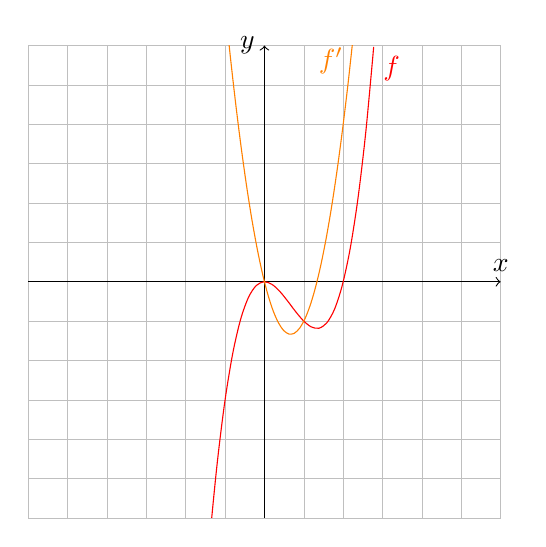
\begin{tikzpicture}[scale=0.5]
      \draw[very thin,lightgray] (-6,-6) grid (6,6);
      \draw[->] (-6,0)--(6,0) node[above]{$x$};
      \draw[->] (0,-6)--(0,6) node[left]{$y$};
      \clip (-6,-6)--(6,-6)--(6,6)--(-6,6)--cycle;
      \draw[red,domain=-2:2.775] plot[smooth] ({\x}, {\x*\x*\x-2*\x*\x})
      node[below right] {$f$};
      \draw[orange,domain=-1:2.25] plot[smooth] (\x,{3*\x*\x-4*\x})
      node[below left] {$f'$};
    \end{tikzpicture}
    \caption{Graphs of $f(x)=x^3-2x^2$ and $f'(x)=3x^2-4x$}
    \label{fig:x3-2x2}
  \end{figure}
\item By the definition of derivative we have
  \begin{align*}
    f(x) &= x^2 - 6x + 5 \\
    f(x+h) &= (x+h)^2-6(x+h)+5 = x^2 +2xh + h^2 - 6x - 6h + 5 \\
    f(x+h)-f(x) &= 2xh + h^2 - 6h \\
    f'(x) &= \lim_{h\to 0} \frac{(2x+h-6)h}{h} = 2x-6
  \end{align*}
  Differentiating the derivative,
  \begin{align*}
    f'(x+h) &= 2x+2h-6 \\
    f'(x+h)-f'(x) &= 2h \\
    f''(x) &= \lim_{h\to 0} \frac{f'(x+h)-f'(x)}{h} 
    = \lim_{h\to 0} \frac{2h}{h} = 2
  \end{align*}
  Differentiating the second derivative,
  \begin{equation*}
    f'''(x) = \lim_{h\to 0} \frac{f''(x+h)-f''(x)}{h} 
    = \lim_{h\to 0} \frac{2-2}{h} = 0
  \end{equation*}
  Differentiating the third derivative,
  \begin{equation*}
    f^{(4)} (x) = \lim_{h\to 0} \frac{f'''(x+h)-f'''(x)}{h}
    = \lim_{h\to 0} \frac{0-0}{h} = 0
  \end{equation*}
  See Figure~\ref{fig:x2-6x+5}.  The function is in red, the first
  derivative in orange, the second derivative in yellow, and the third
  and higher derivatives in green.  Note that where \(f\) is
  decreasing, \(f'\) is negative, and where \(f\) is increasing,
  \(f'\) is positive.  Similar relationships hold between \(f'\) and
  \(f''\), etc.
  \begin{figure}[htbp]
    \centering
    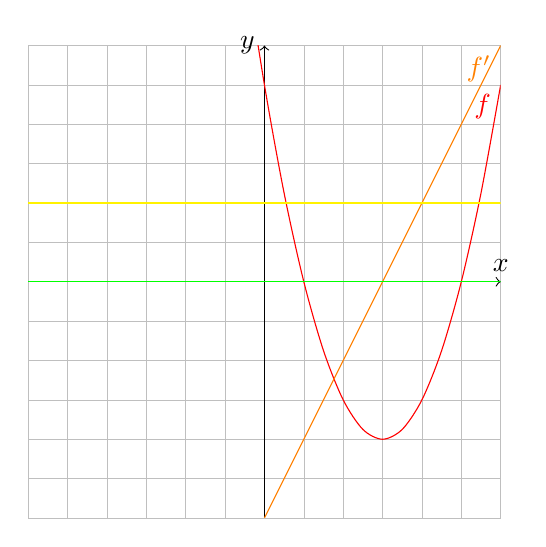
\begin{tikzpicture}[scale=0.5]
      \draw[very thin,lightgray] (-6,-6) grid (6,6);
      \draw[->] (-6,0)--(6,0) node[above]{$x$};
      \draw[->] (0,-6)--(0,6) node[left]{$y$};
      \clip (-6,-6)--(6,-6)--(6,6)--(-6,6)--cycle;
      \draw[red,domain=-6:6] plot[smooth] (\x,{\x*\x-6*\x+5})
      node[below left] {$f$};
      \draw[orange,domain=-6:6] plot[smooth] (\x,{2*\x-6})
      node[below left] {$f'$};
      \draw[yellow] (-6,2)--(6,2);
      \draw[green] (-6,0)--(6,0);
    \end{tikzpicture}
    \caption{Graphs of $f(x)=x^2-6x+5$, $f'(x)=2x-6$, $f''(x)=2$,
      $f'''(x)=0$, $f^{(4)}(x)=0$}
    \label{fig:x2-6x+5}
  \end{figure}
\item See Figure~\ref{fig:cosx} for the graph of $\cos x$ in red and
  its derivative in orange.  The derivative appears to be another
  trigonometric function, a shifted version of the cosine function.
  We will learn more about it in Section~2.4.
  \begin{figure}[htbp]
    \centering
    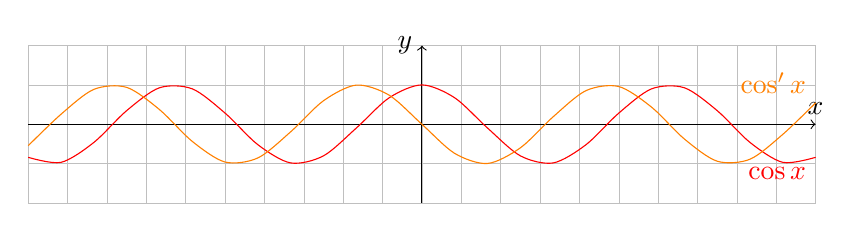
\begin{tikzpicture}[scale=0.5]
      \draw[very thin,lightgray] (-10,-2) grid (10,2);
      \draw[->] (-10,0)--(10,0) node[above]{$x$};
      \draw[->] (0,-2)--(0,2) node[left]{$y$};
      %\clip (-6,-6)--(6,-6)--(6,6)--(-6,6)--cycle;
      \draw[red,domain=-10:10] plot[smooth] ({\x},{cos(deg(\x))})
      node[below left] {$\cos x$};
      \draw[orange,domain=-10:10] plot[smooth] ({\x},{-sin(deg(\x))})
      node[above left] {$\cos' x$};
    \end{tikzpicture}
    \caption{Graphs of $\cos x$ and its derivative}
    \label{fig:cosx}
  \end{figure}
\item The function $y=x^{2/3}$ has a cusp at $(0,0)$, but is
  differentiable at $(8,4)$.  Zooming in on the cusp with an online
  calculator like Desmos, the graph will eventually look like a
  vertical half-line; since the zoomed-in graph does not look like a
  whole line (and since the zoomed-in graph is vertical) we know that
  the function is not differentiable at \((0,0)\).  Zooming in on the
  point \((8,4)\), the function will eventually look like a whole
  non-vertical line, which means that the function is differentiable
  at \((8,4)\).
\item\label{prob:absx-xprime}
  Note that if $x<0$, $|x|=-x$, so $f(x)=|x|-x=-x-x=-2x$; if $x=0$
  then $f(0)=|0|-0=0-0=0$; and if $x>0$ then $|x|=x$ so
  $f(x)=|x|-x=x-x=0$.  In summary, we can write
  \begin{equation*}
    f(x) = \begin{cases} 
      -2x & \mbox{if $x<0$} \\
      0   & \mbox{if $x=0$} \\
      0   & \mbox{if $x>0$}
    \end{cases}
  \end{equation*}
  According to the definition of derivative,
  \begin{equation*}
    f'(0) = \lim_{h\to 0} \frac{f(0+h)-f(0)}{h}
    = \lim_{h\to 0} \frac{f(h)}{h}
  \end{equation*}
  It is difficult to work with $f(h)=|h|-h$ as it was given in the
  problem statement, but we note by the above discussion that $f(h)$
  has simpler expressions when $h<0$ and when $h>0$, so we analyze the
  above limit using one-sided limits.
  \begin{equation*}
    \lim_{h\to 0^-} \frac{f(h)}{h} = 
    \lim_{h\to 0^-} \frac{-2h}{h} = -2
  \end{equation*}
  while on the other hand
  \begin{equation*}
    \lim_{h\to 0^+} \frac{f(h)}{h} = 
    \lim_{h\to 0^+} \frac{0}{h} = 0
  \end{equation*}
  Since the left and right-sided limits do not agree, the two sided
  limit does not exist, so $f(x)$ is not differentiable at $x=0$.

  If $x<0$ then 
  \begin{equation*}
    f'(x) = \lim_{h\to 0} \frac{f(x+h)-f(x)}{h}
    = \lim_{h\to 0} \frac{-2(x+h)-(-2x)}{h} 
    = \lim_{h\to 0} \frac{-2h}{h} = -2
  \end{equation*}
  because we can assume that $x<0$ implies $x+h<0$ for small values of
  $h$ in the limit $h\to 0$, and so $f(x+h) = -2(x+h)$.
  If $x>0$ then similar reasoning shows $f'(x)=0$.  In summary, we
  have
  \begin{equation*}
    f'(x) = \begin{cases}
      -2           & \mbox{if $x<0$} \\
      \mbox{undef} & \mbox{if $x=0$} \\
      0            & \mbox{if $x>0$}
    \end{cases}
  \end{equation*}
  See Figure~\ref{fig:absx-xprime} for the graph of $f'(x)$.
  \begin{figure}[htbp]
    \centering
    $\begin{array}{c@{\hspace{0.5in}}c}
      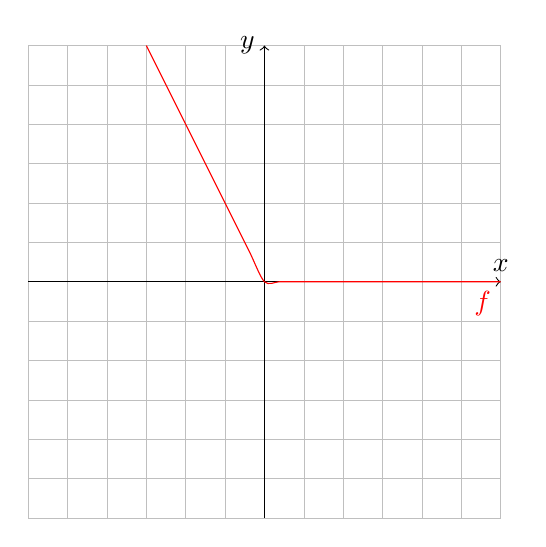
\begin{tikzpicture}[scale=0.5]
        \draw[very thin,lightgray] (-6,-6) grid (6,6);
        \draw[->] (-6,0)--(6,0) node[above]{$x$};
        \draw[->] (0,-6)--(0,6) node[left]{$y$};
        \draw[red,domain=-3:6] plot[smooth] ({\x}, {abs(\x)-\x})
        node[below left] {$f$};
      \end{tikzpicture}
      &
      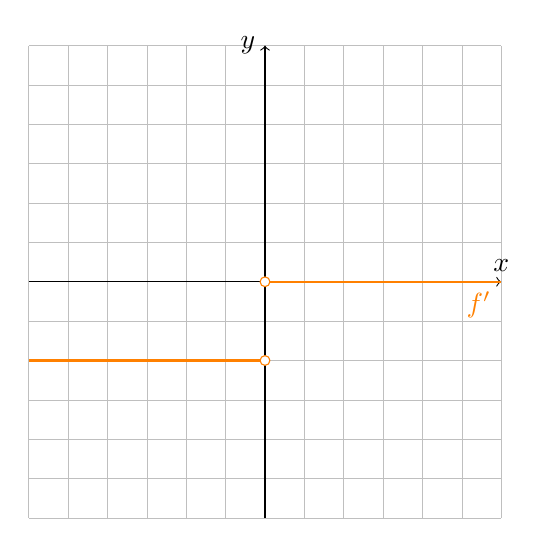
\begin{tikzpicture}[scale=0.5]
        \draw[very thin,lightgray] (-6,-6) grid (6,6);
        \draw[->] (-6,0)--(6,0) node[above]{$x$};
        \draw[->] (0,-6)--(0,6) node[left]{$y$};
        \draw[orange,thick] (-6,-2)--(0,-2);
        \draw[orange,thick] (0,0)--(6,0)
        node[below left] {\(f'\)};
        \node[draw=orange,fill=white,inner sep=1.25pt,shape=circle] at
        (0,-2) {};
        \node[draw=orange,fill=white,inner sep=1.25pt,shape=circle] at
        (0,0) {};
      \end{tikzpicture}
    \\
    \mbox{(a) Graph of $y=f(x)=|x|-x$}
    &
    \mbox{(b) Graph of $y=f'(x)$ where $f(x)=|x|-x$}
    \end{array}$
    \caption{Graphs for Problem~\ref{prob:absx-xprime}}
    \label{fig:absx-xprime}
  \end{figure}
%% \item %4
%%   \begin{enumerate}
%%   \item First write
%%     \begin{equation*}
%%       f(t) = t^{1/2} - t^{-1/2}
%%     \end{equation*}
%%     Using the difference rule
%%     \begin{equation*}
%%       \frac{d}{dt} f(t)
%%       = \frac{d}{dt} \left( t^{1/2} - t^{-1/2} \right)
%%       = \frac{d}{dt} t^{1/2} - \frac{d}{dt} t^{-1/2}
%%     \end{equation*}
%%     Now using the power rule twice,
%%     \begin{equation*}
%%       \frac{d}{dt} f(t) = \frac{1}{2} t^{1/2-1} - \left(-\frac{1}{2}\right)
%%       t^{-1/2-1}
%%       = \frac{1}{2} t^{-1/2} + \frac{1}{2} t^{-3/2}
%%     \end{equation*}
%%   \item Using the constant multiple rule,
%%     \begin{equation*}
%%       \frac{d}{dy} B(y) = \frac{d}{dy} cy^{-6} = c \frac{d}{dy} y^{-6}
%%     \end{equation*}
%%     Using the power rule,
%%     \begin{equation*}
%%       \frac{d}{dy} B(y) = c (-6) y^{-6-1} = -6c y^{-7}
%%     \end{equation*}
%%   \item First we simplify a little:
%%     \begin{equation*}
%%       g(u) = \sqrt{2} u + \sqrt{3u} = \sqrt{2} u + \sqrt{3} \sqrt{u}
%%       = \sqrt{2} u^1 + \sqrt{3} u^{1/2}
%%     \end{equation*}
%%     Using the sum rule,
%%     \begin{equation*}
%%       \frac{d}{du} g(u) 
%%       = \frac{d}{du} \left( \sqrt{2} u^1 + \sqrt{3} u^{1/2} \right)
%%       = \frac{d}{du} \sqrt{2} u^1 + \frac{d}{du} \sqrt{3} u^{1/2}
%%     \end{equation*}
%%     Using the constant multiple rule
%%     \begin{equation*}
%%       \frac{d}{du} g(u)
%%       = \sqrt{2} \frac{d}{du} u^1 + \sqrt{3} \frac{d}{du} u^{1/2}
%%     \end{equation*}
%%     Finally, using the power rule,
%%     \begin{equation*}
%%       \frac{d}{du} g(u) 
%%       = \sqrt{2} 1 u^{1-1} + \sqrt{3} \frac{1}{2} u^{1/2-1}
%%       = \sqrt{2} + \frac{\sqrt{3}}{2} u^{-1/2}
%%     \end{equation*}
%%   \item First, we write the powers in exponential notation and
%%     expand the square to obtain
%%     \begin{equation*}
%%       v = \left( x^{1/2} + x^{-1/3} \right)^2
%%       = x^{1/2})^2 + 2 x^{1/2} x^{-1/3} + (x^{-1/3})^2
%%       = x + 2x^{1/6} + x^{-2/3}
%%     \end{equation*}
%%     Now we use the sum and constant multiple rules to obtain
%%     \begin{equation*}
%%       \frac{dv}{dx} = \frac{d}{dx} \left( x + 2x^{1/6} + x^{-2/3} \right)
%%       = \frac{d}{dx} x + 2 \frac{d}{dx} x^{1/6} + \frac{d}{dx} x^{-2/3}
%%     \end{equation*}
%%     and the power rule to obtain
%%     \begin{equation*}
%%       \frac{dv}{dx} = 1 + 2 \frac{1}{6} x^{1/6-1} + \left(-\frac{2}{3}\right)
%%         x^{-2/3-1}
%%       = 1 + \frac{1}{3} x^{-5/6} - \frac{2}{3} x^{-5/3}
%%     \end{equation*}
%%   \end{enumerate}
%% \item %4
%%   We use the quotient rule first in all of the parts of this question
%%   \begin{enumerate}
%%   \item 
%%     We have
%%     \begin{equation*}
%%       f'(t) = \frac{d}{dt} \frac{2t}{4+t^2}
%%       = \frac{(4+t^2) \frac{d}{dt} 2t - 2t \frac{d}{dt} (4+t^2)}{(4+t^2)^2}
%%       = \frac{(4+t^2)(2) - 2t (2t)}{(4+t^2)^2}
%%     \end{equation*}
%%     where we have used the sum, constant multiple, and power rules in the
%%     last step above.  Further simplification is possible, but is not necessary
%%     in this question:
%%     \begin{equation*}
%%       f'(t) = \frac{8 + 2t^2 - 4t^2}{(4+t^2)^2}
%%       = \frac{8-2t^2}{(4+t^2)^2}
%%     \end{equation*}
%%   \item By the quotient rule,
%%     \begin{equation*}
%%       \frac{dy}{dx} = \frac{(x^3+x-3)\frac{d}{dx}(x+1) - (x+1) \frac{d}{dx} 
%%         (x^3+x-3)}{(x^3+x-3)^2}
%%       = \frac{(x^3-x-3)(1) - (x+1) (3x^2+1)}{(x^3+x-3)^2}
%%     \end{equation*}
%%     Further simplification is optional:
%%     \begin{equation*}
%%       \frac{dy}{dx} = \frac{x^3-x-3-3x^3-x-3x^2-1}{(x^3+x-3)^2}
%%       = \frac{-2x^3-3x^2-2x-4}{(x^3+x-3)^2}
%%     \end{equation*}
%%     Note that I have not expanded the denominator, which is seldom a useful
%%     simplification.
%%   \item By the quotient rule,
%%     \begin{equation*}
%%       \frac{dy}{dt} = \frac{(t-1)^2\frac{d}{dt} t - t \frac{d}{dt} (t-1)^2}{
%%         ((t-1)^2)^2}
%%     \end{equation*}
%%     In order to take the derivative of $(t-1)^2$ in the above expression
%%     we must first expand it (in the numerator, not the denominator) to
%%     obtain
%%     \begin{equation*}
%%       \frac{dy}{dt} = \frac{(t-1)^2\frac{d}{dt} t - t \frac{d}{dt}(t^2-2t+1)}{
%%         ((t-1)^2)^2}
%%       = \frac{(t-1)^2(1) - t (2t-2)}{(t-1)^4}
%%     \end{equation*}
%%     where we have used the rules of exponents in the denominator.
%%     Further simplification is optional:
%%     \begin{equation*}
%%       \frac{dy}{dt} = \frac{t^2-2t+1-2t^2+2t}{(t-1)^4}
%%       = \frac{1-t^2}{(t-1)^4}
%%     \end{equation*}
%%   \item We write all the powers in exponential notation and then
%%     apply the quotient rule:
%%     \begin{align*}
%%       g'(t) 
%%       &= \frac{d}{dt} \frac{t-t^{1/2}}{t^{1/3}}
%%       = \frac{t^{1/3} \frac{d}{dt} (t-t^{1/2}- (t-t^{1/2})\frac{d}{dt} t^{1/3}}{
%%         (t^{1/3})^2}
%%       \\
%%       &= \frac{t^{1/3} (1-(1/2)t^{-1/2}) - (t-t^{1/2}) (1/3) t^{-2/3}}{t^{2/3}}
%%     \end{align*}
%%     Further simplification is optional but is not necessary.  First we clear
%%     fractions by multiplying the numerator and denominator through by $6$:
%%     \begin{equation*}
%%       g'(t) = \frac{t^{1/3} (6-3t^{-1/2}) - (t-t^{1/2}) 2 t^{-2/3}}{t^{2/3}}
%%       = \frac{6t^{1/3} - 3t^{-1/6} - 2t^{1/3}+2t^{-1/6}}{t^{2/3}}
%%     \end{equation*}
%%   \end{enumerate}
%% \item %5
%%   We are given a point on the tangent line, so we must find its slope in order
%%   to write the equation in point-slope form.
%%   \begin{enumerate}
%%   \item By habit, I first do the optional check that the given point is
%%     actually on the line: when $x=1$, $y=(1+2(1))^2=3^2=9$, so the point
%%     $(1,9)$ actually is on the line.  To find the slope, we 
%%     expand then differentiate:
%%     \begin{equation*}
%%       y = (1+2x)^2 = 1 + 4x + 4x^2 \implies
%%       y' = 4 + 8x
%%     \end{equation*}
%%     so $y'(1) = 4+8(1)= 12$, i.e., the slope of the tangent line at the point
%%     $(x,y)=(1,9)$ is $y'(1)=12$.  Then the equation of the tangent line in 
%%     point-slope form is
%%     \begin{equation*}
%%       y-9 = 12 (x-1)
%%     \end{equation*}
%%     Further simplification is possible but is not necessary.  Finally, if the
%%     slope of a line is $12$, the slope of the perpendicular line is the
%%     negative reciprocal of $12$, i.e., $-1/12$, so the equation of the normal
%%     line is
%%     \begin{equation*}
%%       y-9 = -\frac{1}{12} (x-1)
%%     \end{equation*}
%%   \item We have
%%     \begin{equation*}
%%       y(4) = \frac{\sqrt{4}}{4+1} = \frac{2}{5} = 0.4
%%     \end{equation*}
%%     so the point $(4,0.4)$ actually is a point on the curve.  The slope of
%%     the tangent line at that point is found by taking the derivative:
%%     \begin{equation*}
%%       y'(x) = \frac{(x+1) \frac{d}{dx} x^{1/2} - x^{1/2} \frac{d}{dx} (x+1)}{
%%         (x+1)^2}
%%       = \frac{(x+1) (1/2) x^{-1/2} - x^{1/2} (1)}{(x+1)^2}
%%     \end{equation*}
%%     so 
%%     \begin{equation*}
%%       y'(4) = \frac{5(1/2)(1/2) - 2}{25} = \frac{5-8}{100} = -\frac{3}{100}
%%     \end{equation*}
%%     Therefore the equation of the tangent line is
%%     \begin{equation*}
%%       y-\frac{2}{5} = -\frac{3}{100} (x-4)
%%     \end{equation*}
%%     and the equation of the normal line, which has the same point but 
%%     negative reciprocal slope, is
%%     \begin{equation*}
%%       y-\frac{2}{5} = \frac{100}{3} (x-4)
%%     \end{equation*}
%%   \end{enumerate}
%% \item %6
%%   \begin{enumerate}
%%   \item Write $G(r)=r^{1/2} + r^{1/3}$.  Then by the sum and power rules,
%%     $G'(r)=(1/2) r^{-1/2} + (1/3) r^{-2/3}$.  Differentiating again, by the
%%     sum, constant multiple, and power rules, $G''(r) = (1/2)(-1/2) r^{-3/2}
%%     + (1/3)(-2/3) r^{-5/3}$.  Simplification is optional:
%%     $G''(r)=-(1/4)r^{-3/2} - (2/9) r^{-5/3}$.
%%   \item By the quotient rule,
%%     \begin{equation*}
%%       f'(x) = \frac{(3-x)\frac{d}{dx} 1 - 1 \frac{d}{dx} (3-x)}{(3-x)^2}
%%       = \frac{1}{(3-x)^2}
%%     \end{equation*}
%%     Differentiating again, by the quotient rule,
%%     \begin{equation*}
%%       f''(x) = \frac{(3-x)^2\frac{d}{dx} 1 - 1 \frac{d}{dx}(3-x)^2}{(3-x)^4}
%%       = \frac{-\frac{d}{dx}(9-6x+x^2)}{(3-x)^4}
%%       = \frac{6-2x}{(3-x)^4}
%%     \end{equation*}
%%     Some optional simplification is possible:
%%     \begin{equation*}
%%       f''(x) = \frac{2(3-x)}{(3-x)^4} = \frac{2}{(3-x)^3}
%%     \end{equation*}
%%     You can check the result using the chain rule, if you know it.
%%   \end{enumerate}
%% \item \label{prob:parallel} 
%%   Two lines are parallel if and only if they have the same slope.  The 
%%   slope of the line $x-2y=2$ can be obtained by solving for $y$ and examining
%%   the coefficient of $x$: $2y=x-2$, $y=(1/2)x-1$, so the slope of the given
%%   line is $1/2$, hence the slope of all parallel lines is $1/2$, and we are
%%   looking for tangent lines with slope $1/2$.

%%   The slope of a tangent line to the given curve can be obtained by taking
%%   the derivative:
%%   \begin{equation*}
%%     y' = \frac{(x+1)\frac{d}{dx} (x-1) - (x-1)\frac{d}{dx} (x+1)}{(x+1)^2}
%%     = \frac{(x+1)-(x-1)}{(x+1)^2} = \frac{2}{(x+1)^2}
%%   \end{equation*}
%%   We are looking for $x$ values at which $y'=1/2$; in other words, we want
%%   to solve the equation
%%   \begin{equation*}
%%     y' = 1/2 \implies \frac{2}{(x+1)^2}=1/2 \implies
%%     (x+1)^2=4 \implies x+1 = \pm 2 \implies x=1,-3
%%   \end{equation*}
%%   The number $x=1$ gives the point on the curve $(1,y(1))=(1,0)$ and of course
%%   slope $y'(1)=1/2$, so the equation of the tangent line is $y-0=(1/2)(x-1)$.
%%   The other number $x=-3$ gives the point on the curve $(-3,2)$ and tangent
%%   line $y-2=(1/2)(x+3)$.  See Figure~\ref{fig:parallel}.
%%   \begin{figure}[htbp]
%%     \centering
%%     \begin{tikzpicture}
%%       \draw[gray,very thin] (-4,-4) grid (4,4);
%%       \draw[->] (-4,0)--(4,0);
%%       \draw[->] (0,-4)--(0,4);
%%       % function is y=1-2/(x+1), inverse x=-1+2/(1-y) 
%%       % x=-4 -> y=5/3 ok
%%       % x=4  -> y=3/5 ok
%%       % y=4  -> x=-5/3
%%       % y=-4 -> x=-3/5
%%       \draw[color=red,domain=-4:-1.666] plot(\x,{(\x-1)/(\x+1)});
%%       \draw[color=red,domain=-0.6:4] plot(\x,{(\x-1)/(\x+1)}) node[right] {$y=\frac{x-1}{x+1}$};
%%       \draw[color=blue,domain=-4:4] plot(\x,{\x/2 - 1}) node[right] {$x-2y=2$};
%%       \draw[color=blue,domain=-4:1] plot(\x,{0.5*(\x+3)+2}) node[right] {$y-2=\frac{1}{2}(x+3)$};
%%     \end{tikzpicture}
%%     \caption{Graph for Problem~\ref{prob:parallel}}
%%     \label{fig:parallel}
%%   \end{figure}
%% \item \label{prob:2tans} %8 FIXME diagrams!
%%   Let $(a,a^2+a)$ be a point on the parabola.  The slope at that point is
%%   $2a+1$, so the equation of any tangent line to the parabola is 
%%   $y-(a^2+a) = (2a+1)(x-a)$.
%%   \begin{enumerate}
%%   \item For a tangent line to pass through $(2,-3)$ we must have
%%     $-3-(a^2+a) = (2a+1) (2-a)$ which implies
%%     $-3-a^2-a = 4a+2-2a^2-a$ or $a^2-4a-5=0$ or $(a+1)(a-5)=0$, $a=-1,5$.
%%     You should check that both of those values of $a$ give tangent lines
%%     passing through the given point.
%%   \item For a tangent line to pass through $(2,7)$ we must have
%%     $7-(a^2+a)=(2a+1)(2-a)$ or $7-a^2-a=4a+2-2a^2-a$ or
%%     $a^2-4a+5=0$.  That equation does not have a solution for $a$ because
%%     its discriminant $\Delta=-(-4)-4(1)(5)=4-20=-16<0$.
%%   \end{enumerate}
%%   See Figure~\ref{fig:2tans}.
%%   \begin{figure}[htbp]
%%     \centering
%%     $\begin{array}{c@{\hspace{0.5in}}c}
%%     \begin{tikzpicture}[scale=0.5]
%%       \draw[gray,very thin] (-5,-5) grid (5,5);
%%       \draw[->] (-5,0)--(5,0);
%%       \draw[->] (0,-5)--(0,5);
%%       \draw[color=red,domain=-5:5] plot(\x,{(\x*\x+\x)/10}); % node[left] {$y=x^2+x$};
%%       \draw[color=blue,domain=-5:5] plot(\x,{(-\x-1)/10});
%%       \draw[color=blue,domain=-2.273:5] plot(\x,{1.1*(\x-5)+3});
%%       \node[fill=blue,minimum size=3pt,inner sep=1pt] at (2,-3/10) {};
%%       % 1.1(x-5)+3=-5 -> 1.1(x-5)=-8 -> (x-5)=-8/1.1 -> x=5-8/1.1 = -2.273
%%     \end{tikzpicture}
%%     &
%%     \begin{tikzpicture}[scale=0.5]
%%       \draw[gray,very thin] (-5,-5) grid (5,5);
%%       \draw[->] (-5,0)--(5,0);
%%       \draw[->] (0,-5)--(0,5);
%%       \draw[color=red,domain=-5:5] plot(\x,{(\x*\x+\x)/10}); % node[left] {$y=x^2+x$};
%%       \node[fill=blue,minimum size=3pt,inner sep=1pt] at (2,8/10) {};
%%     \end{tikzpicture}
%%     \\
%%     \mbox{(a) Point with two tangents}
%%     &
%%     \mbox{(b) Point with no tangents}
%%     \end{array}$
%%     \caption{Graphs for Problem~\ref{prob:2tans}}
%%     \label{fig:2tans}
%%   \end{figure}
\item \label{prob:1323} 
  \begin{enumerate}
  \item Write $f(x)=x^{1/3}$.  Then $f'(x)=(1/3)x^{-2/3}$.
  \item By the result above, $f'(x)$ is undefined for $x=0$ because of the
    negative power of $x$.
  \item To show that $f(x)$ has a vertical tangent at $x=0$, we need to
    perform a more careful analysis of the derivative of $f(x)$ at $x=0$
    using the definition of the derivative.  We have
    \begin{equation*}
      f'(0) = \lim_{h\to 0} \frac{f(0+h)-f(0)}{h}
      = \lim_{h\to 0} \frac{h^{1/3}-0}{h}
      = \lim_{h\to 0} h^{-2/3} = +\infty
    \end{equation*}
    because $h^{-2/3}=1/(h^{1/3})^2$ is a large positive number when
    $h$ is a small positive or negative number.  Since $f'(0)=+\infty$ we
    have a vertical tangent, a tangent with slope $+\infty$.

    Compare the above result to the result for $g(x)=x^{2/3}$, which
    does not have a vertical tangent at $x=0$ but instead has a cusp.
    See Figure~\ref{fig:1323}.
  \end{enumerate}
  \begin{figure}[htbp]
    \centering
    $\begin{array}{c@{\hspace{0.5in}}c}
    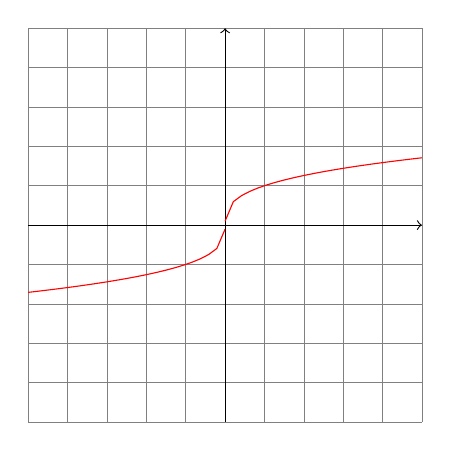
\begin{tikzpicture}[scale=0.5]
      \draw[gray,very thin] (-5,-5) grid (5,5);
      \draw[->] (-5,0)--(5,0);
      \draw[->] (0,-5)--(0,5);
      \draw[color=red,domain=-5:-0.001] plot(\x,{(-1)*(abs(\x))^(0.333)}); % node[left] {$y=x^2+x$};
      \draw[color=red,domain=0.001:5] plot(\x,{(abs(\x))^(0.333)}); % node[left] {$y=x^2+x$};
    \end{tikzpicture}
    &
    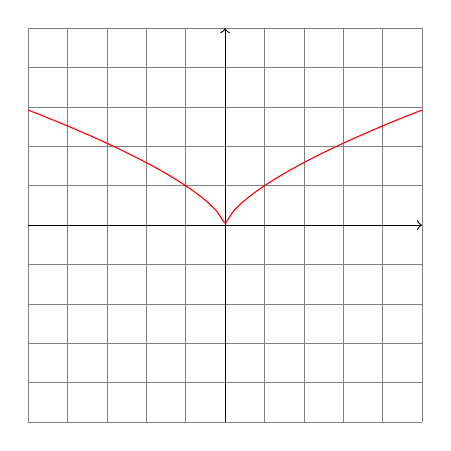
\begin{tikzpicture}[scale=0.5]
      \draw[gray,very thin] (-5,-5) grid (5,5);
      \draw[->] (-5,0)--(5,0);
      \draw[->] (0,-5)--(0,5);
      \draw[color=red,domain=-5:-0.01] plot(\x,{(abs(\x))^(0.666)}); % node[left] {$y=x^2+x$};
      \draw[color=red,domain=0.01:5] plot(\x,{(abs(\x))^(0.666)}); % node[left] {$y=x^2+x$};
    \end{tikzpicture}
    \\
    \mbox{(a) Graph of $y=x^{1/3}$}
    &
    \mbox{(b) Graph of $y=x^{2/3}$}
    \end{array}$
    \caption{Graphs for Problem~\ref{prob:1323}}
    \label{fig:1323}
  \end{figure}
%% \item \label{prob:piece} %10 FIXME diagrams!
%%   The function $g(x)$ is piecewise defined on the pieces $x<-1$,
%%   $-1\le x \le 1$, and $1<x$.  The function is differentiable in the 
%%   interiors of those intervals, with derivative found by the usual
%%   differentiation rules, so we have
%%   \begin{equation*}
%%     g'(x) = \begin{cases}
%%       -2 &\mbox{if $x<-1$} \\
%%       ?  &\mbox{if $x=-1$} \\
%%       2x &\mbox{if $-1<x<1$} \\
%%       ?  &\mbox{if $x=1$}    \\
%%       1  &\mbox{if $1<x$}
%%     \end{cases}
%%   \end{equation*}
%%   The only numbers in question are $x=-1$ and $x=1$, the boundaries between
%%   the pieces.  We need to check the differentiability of $g(x)$ using the
%%   definition of the derivative.

%%   At $x=-1$ we have
%%   \begin{equation*}
%%     g'(-1) = \lim_{h\to 0} \frac{g(-1+h)-g(-1)}{h}
%%     = \lim_{h\to 0} \frac{g(-1+h)-(-1)^2}{h}
%%     = \lim_{h\to 0} \frac{g(-1+h)-1}{h}
%%   \end{equation*}
%%   Since $g(x)$ takes on different forms to the left and to the right of $x=-1$,
%%   we must use one-sided limits to make progress with the above limit.  We have
%%   \begin{equation*}
%%     \lim_{h\to 0^-} \frac{g(-1+h)-1}{h}
%%     = \lim_{h\to 0^-} \frac{-1-2(-1+h)-1}{h}
%%     = \lim_{h\to 0^-} \frac{-2+2-2h}{h} = -2
%%   \end{equation*}
%%   where we have used the formula $g(-1+h)=-1-2(-1+h)$ because $-1+h<-1$ when
%%   $h\to 0^-$.  On the other hand,
%%   \begin{equation*}
%%     \lim_{h\to 0^+} \frac{g(-1+h)-1}{h}
%%     = \lim_{h\to 0^+} \frac{(-1+h)^2-1}{h}
%%     = \lim_{h\to 0^+} \frac{1-2h+h^2-1}{h}
%%     = -2
%%   \end{equation*}
%%   so the two one-sided limits agree, which means that the two-sided limit
%%   exists and equals $-2$ in value.  In other words,
%%   \begin{equation*}
%%     g'(-1) = \lim_{h\to 0} \frac{g(-1+h)-g(-1)}{h}
%%     = \lim_{h\to 0} \frac{g(-1+h)-(-1)^2}{h}
%%     = \lim_{h\to 0} \frac{g(-1+h)-1}{h}
%%     = -2
%%   \end{equation*}

%%   Similarly, at $x=1$, we have
%%   \begin{equation*}
%%     g'(1) = 
%%     \lim_{h\to 0} \frac{g(1+h)-g(1)}{h}
%%     = \lim_{h\to 0} \frac{g(1+h)-(1)^2}{h}
%%     = \lim_{h\to 0} \frac{g(1+h)-1}{h}
%%   \end{equation*}
%%   Again, to evaluate the limit, we have to look at the one-sided limits 
%%   separately.  We have
%%   \begin{equation*}
%%     \lim_{h\to 0^-} \frac{g(1+h)-1}{h}
%%     = \lim_{h\to 0^-} \frac{(1+h)^2-1}{h}
%%     = \lim_{h\to 0^-} \frac{1+2h+h^2-1}{h}
%%     = 2
%%   \end{equation*}
%%   but
%%   \begin{equation*}
%%     \lim_{h\to 0^+} \frac{g(1+h)-1}{h}
%%     = \lim_{h\to 0^+} \frac{(1+h)-1}{h}
%%     = 1
%%   \end{equation*}
%%   so the one-sided limits don't agree, hence the two-sides limit doesn't
%%   exist, i.e., $g'(1)$ doesn't exist.  (The point $x=1$ is an ``angle point''
%%   for the function because the one-sided derivatives exist but are not
%%   equal.)  So we can complete our tabulation of the derivative of $g(x)$ as
%%   follows:
%%   \begin{equation*}
%%     g'(x) = \begin{cases}
%%       -2               &\mbox{if $x<-1$}   \\
%%       -2               &\mbox{if $x=-1$}   \\
%%       2x               &\mbox{if $-1<x<1$} \\
%%       \mbox{undefined} &\mbox{if $x=1$}    \\
%%       1                &\mbox{if $1<x$}
%%     \end{cases}
%%   \end{equation*}
%%   See Figures \ref{fig:pieceg}~and~\ref{fig:piecegp}.  Note that the pieces of 
%%   $g(x)$ come together from different directions at $x=1$, so there is an
%%   angle point at $x=1$, not differentiable.  On the other hand, the two pieces
%%   of $g(x)$ join together in exactly the right direction at $x=-1$, and the
%%   function is differentiable there.
%%   \begin{figure}[htbp]
%%     \centering
%%     \begin{tikzpicture}
%%       \draw[gray,very thin] (-5,-1) grid (5,5);
%%       \draw[->] (-5,0)--(5,0);
%%       \draw[->] (0,-1)--(0,5);
%%       \draw[color=red,domain=-3:-1] plot(\x,{-1-2*\x}); % node[left] {$y=x^2+x$};
%%       \draw[color=red,domain=-1:1] plot(\x,{(\x)^2}); % node[left] {$y=x^2+x$};
%%       \draw[color=red,domain=1:5] plot(\x,{\x}); % node[left] {$y=x^2+x$};
%%     \end{tikzpicture}
%%     \caption{Graph of $g(x)$ for Problem~\ref{prob:piece}}
%%     \label{fig:pieceg}
%%   \end{figure}
%%   \begin{figure}
%%     \centering
%%     \begin{tikzpicture}
%%       \draw[gray,very thin] (-5,-2) grid (5,5);
%%       \draw[->] (-5,0)--(5,0);
%%       \draw[->] (0,-2)--(0,5);
%%       \draw[color=red,thick,domain=-5:-1] plot(\x,{-2}); % node[left] {$y=x^2+x$};
%%       \draw[color=red,thick,domain=-1:1] plot(\x,{2*\x}); % node[left] {$y=x^2+x$};
%%       \draw[color=red,thick,domain=1:5] plot(\x,1); % node[left] {$y=x^2+x$};
%%       \node[fill=red,minimum size=3pt, inner sep=1pt] at (-1,-2) {};
%%       \node[draw=red,minimum size=3pt, inner sep=1pt] at (1,2) {};
%%       \node[draw=red,minimum size=3pt, inner sep=1pt] at (1,1) {};
%%     \end{tikzpicture}
%%     \caption{Graph of $g'(x)$ for Problem~\ref{prob:piece}}
%%     \label{fig:piecegp}
%%   \end{figure}
\item First we find out all we can about the tangent line.  We know a
  point on the line, namely $(1,1)$, so all we need is the slope of
  the line to determine the line.  The slope is the derivative of the
  function evaluated at $x=1$, i.e.,
  \begin{equation*}
    f'(1) = \lim_{h\to 0} \frac{f(1+h)-f(1)}{h}
    = \lim_{h\to 0} \frac{(1+h)^2-3(1+h)+3-1}{h} 
    = \lim_{h\to 0} \frac{(2+h-3)h}{h} = -1
  \end{equation*}
  So the equation of the tangent line is 
  \begin{equation*}
    y-y_0 = m(x-x_0) \implies y-1 = (-1) (x-1) \implies y=-x+2
  \end{equation*}
  See Figure~\ref{fig:phi}.  Forming a right triangle with the tangent
  line as hypoteneuse and the angle of inclination as the angle, we
  see that the tangent of the angle of inclination is the opposite
  over the adjacent, or the rise over the run, in other words the
  slope.  In general we have $\tan \phi = m$.  In this case, we have
  $\tan \phi = -1$ so $\phi = \tan^{-1} (-1)$.  My calculator says
  $\phi \approx -0.79$ radians, or $\phi = -45$ degrees.
  \begin{figure}[htbp]
    \centering
    \begin{tikzpicture}[scale=0.5]
      \draw[very thin,lightgray] (-6,6) grid (6,6);
      \draw[->] (-6,0)--(6,0) node[above]{$x$};
      \draw[->] (0,-6)--(0,6) node[left]{$y$};
      \clip (-6,-6)--(-6,6)--(6,6)--(6,-6)--cycle;
      \draw[red,domain=-6:6] plot[smooth] (\x,{\x^2-3*\x+3});
      \node[draw=red,fill=red,inner sep=1.25pt,shape=circle] at
      (1,1) {};
      \draw[red] (-4,6)--(6,-4);
      \draw[blue,->] (3,0) arc (0:-45:1) node[midway,right] {\(\phi\)}; 
      \draw[blue] (5,0)--(5,-3);
    \end{tikzpicture}
    \caption{Graphs of $f(x)=x^2-3x+3$ and Tangent Line}
    \label{fig:phi}
  \end{figure}
\end{enumerate}
\end{document}


